%%%%%%%%%%%%%%%%%%%%%%% file template.tex %%%%%%%%%%%%%%%%%%%%%%%%%
%
% This is a general template file for the LaTeX package SVJour3
% for Springer journals.          Springer Heidelberg 2010/09/16
%
% Copy it to a new file with a new name and use it as the basis
% for your article. Delete % signs as needed.
%
% This template includes a few options for different layouts and
% content for various journals. Please consult a previous issue of
% your journal as needed.
%
%%%%%%%%%%%%%%%%%%%%%%%%%%%%%%%%%%%%%%%%%%%%%%%%%%%%%%%%%%%%%%%%%%%
%
% First comes an example EPS file -- just ignore it and
% proceed on the \documentclass line
% your LaTeX will extract the file if required
\begin{filecontents*}{example.eps}
%!PS-Adobe-3.0 EPSF-3.0
%%BoundingBox: 19 19 221 221
%%CreationDate: Mon Sep 29 1997
%%Creator: programmed by hand (JK)
%%EndComments
gsave
newpath
  20 20 moveto
  20 220 lineto
  220 220 lineto
  220 20 lineto
closepath
2 setlinewidth
gsave
  .4 setgray fill
grestore
stroke
grestore
\end{filecontents*}
%
\RequirePackage{fix-cm}
%
%\documentclass{svjour3}                     % onecolumn (standard format)
%\documentclass[smallcondensed]{svjour3}     % onecolumn (ditto)
\documentclass[smallextended]{svjour3}       % onecolumn (second format)
%\documentclass[twocolumn]{svjour3}          % twocolumn
%
\smartqed  % flush right qed marks, e.g. at end of proof
%

%\usepackage{showframe}
\usepackage{url}
\usepackage{color}
\usepackage{graphics,graphicx}
\usepackage{epsfig}
\usepackage{epstopdf}
\usepackage{colortbl}
\usepackage{multirow}
\usepackage{booktabs}
\usepackage{ifthen}  
\usepackage{rotating}
\usepackage{tabularx}
\usepackage{tabulary}
\usepackage{array}
\usepackage{enumitem}
\usepackage{textcomp}
\usepackage{amsmath}
\usepackage{adjustbox}
\usepackage[]{algorithm2e}
%
% \usepackage{mathptmx}      % use Times fonts if available on your TeX system
%
% insert here the call for the packages your document requires
%\usepackage{latexsym}
% etc.
%
% please place your own definitions here and don't use \def but
% \newcommand{}{}
%
% Insert the name of "your journal" with
% \journalname{myjournal}
%

\newcommand{\ym}[1]{\textcolor{blue}{#1}}
\newcommand{\todo}[1]{\textcolor{red}{#1}}
\newcommand{\anon}[1]{\textcolor{black}{~(anon.)}}
\newcommand{\anoncite}[1]{\textcolor{black}{[anon.]}}

\newcolumntype{D}[1]{>{\centering\arraybackslash}p{#1}}
\newcolumntype{L}[1]{>{\arraybackslash}p{#1}}

\begin{document}

\title{The Impact of Result Diversification on Search Behaviour and Performance}

%\subtitle{Do you have a subtitle?\\ If so, write it here}

%\titlerunning{Short form of title}        % if too long for running head

\author{Maxwell \and
        Azzopardi \and Moshfeghi 
}

%\authorrunning{Short form of author list} % if too long for running head

\institute{David Maxwell \at
              School of Computing Science\\University of Glasgow \\Scotland\\
              \email{d.maxwell.1@research.gla.ac.uk}             \\
%             \emph{Present address:} of F. Author  %  if needed
           \and
           Leif Azzopardi \at
              Department of Computer and Information Sciences\\
              University of Strathclyde\\Scotland\\
              \email{leif.azzopardi@strath.ac.uk} \\
            \and
           Yashar Moshfeghi \at
              Department of Computer and Information Sciences\\
              University of Strathclyde\\Scotland\\
              \email{yashar.moshfeghi@strath.ac.uk} \\    
}

\date{Received: date / Accepted: date}
% The correct dates will be entered by the editor


\maketitle

\begin{abstract}
\emph{Result diversification} aims to provide searchers with a broader view of a given topic, while attempting to maximise the chances of retrieving relevant material. Diversification of results also aims to reduce search bias by increasing the coverage over different aspects of the topic. As such, searchers should learn more about the given topic in general. Despite \emph{diversification} algorithms being introduced over two decades ago, little research has explicitly examined their impact on search behaviour and performance in the context of \emph{Interactive Information Retrieval (IIR)}. In this paper, we explore the impact of diversification when searchers undertake complex search tasks that require learning about different aspects of a topic \emph{(aspectual retrieval)}. For such aspectual retrieval tasks, diversification \emph{should} lead to performance benefits, but does it also lead to improvements on \emph{ad-hoc retrieval} tasks? In addition, how does diversification affect search behaviours and satisfaction? Based on \emph{Information Foraging Theory (IFT)}, we infer two, seemingly counter-intuitive, hypotheses, whereby diversification will lead to searchers examining fewer documents per query, and issue more queries overall. To this end, we performed a within-subjects user study using the \emph{TREC AQUAINT} collection with 51 participants, examining the differences in search performance and behaviour when using: \emph{(i)} a non-diversified system (\emph{BM25}); versus \emph{(ii)} a diversified system (BM25+\emph{xQuAD}) when the search task is either: \emph{(a)} ad-hoc; or \emph{(b)} aspectual. Our results show a number of notable findings in terms of search behaviour, with participants on the diversified system issuing more queries and examining fewer documents per query. Furthermore, we show that when using the diversified system, participants were: more confident about their decisions; more successful; and found a greater number of aspects about the given topics. We also observed that the diversified system was preferred, and led to greater success by participants, regardless of the search task. This work shows that searchers' behaviours (and thus the user model by which we evaluate retrieval systems) changes depending upon the retrieval algorithm and task. This work motivates further research into complex search tasks such as aspectual retrieval -- and how diversity can play an important role in improving the search experience, as well as potentially mitigating bias in search results.


\keywords{\todo{Diversification \and User Study \and User Behavior (what keywords did you use?)}}
% \PACS{PACS code1 \and PACS code2 \and more}
% \subclass{MSC code1 \and MSC code2 \and more}
\end{abstract}

%!TEX root = jir2018aspects.tex
\section{Introduction} \label{sec:intro}
\emph{Interactive Information Retrieval (IIR)} is a complex (and often exploratory) process~\cite{ingwersen2005theturn} in which a searcher issues a variety of queries as a means to explore the topic space~\cite{kelly2015search_tasks}. Often, such tasks are \emph{aspectual} in nature, where an underlying goal is to find out about the different facets, dimensions or aspects of the topic. This type of task is often referred to as \emph{aspectual retrieval}. While aspectual retrieval has been heavily studied in the past (during the TREC Interactive Tracks~\cite{over2001trec}), there has been renewed interest in the search task as it represents a novel context to explore the idea of \emph{``search as learning''}~\cite{collins2017sal}. In this context, the goal of the system is to help the searcher learn about a topic~\cite{collins2017sal} -- and in doing so, the number of aspects that the searcher finds indicates how much they learned during the process~\cite{syed2017sal}. If the goal is to help people learn about a topic, then by returning results that are more diverse in nature and presenting a broader view on the topic, these changes \emph{should} help searchers learn more about the said topic. This reasoning suggests that employing \emph{diversification} will lead to an improved search and learning experience~\cite{syed2017sal}. 

While there have been numerous diversification algorithms developed and proposed over the years~\cite{carbonell1998mmr,chen2006lessismore,santos2010query_reformulations_diversification,santos2011intent,zhai2015subtopics}, the focus here has been on addressing the problem of intents, rather than how diversification affects complex search tasks, such as \emph{ad-hoc} or aspectual retrieval. In this paper, we perform one of the first investigations into the influence and impact of result diversification on search behaviour and search performance when performing different search tasks (ad-hoc or aspectual). Our focus is on understanding how behaviours -- in particular, how searching and stopping behaviours -- change under the different conditions. We ground our study by drawing upon \emph{Information Foraging Theory (IFT)}~\cite{pirolli1999ift} (see Section~\ref{sec:background}) which derives the following hypotheses regarding diversification when performing aspectual search tasks: \emph{(i)} diversification will lead to searchers examining fewer documents per query; and either \emph{(ii)} issuing more queries, or \emph{(iii)} completing the task in less time. However, these hypotheses seem to be counter to our intuition. If a system provides a more diversified set of results, then searchers \emph{should} be able to exploit the diversification of results and find more varied aspects by examining more documents for a given query -- and thus issue fewer queries. In order to explore the validity of the IFT hypotheses and test our intuitions, we designed a $2 \times 2$ within-subjects user study, where participants were tasked to learn about four different topics under the following conditions, using: \emph{(i)} a non-diversified system (\emph{BM25}); versus \emph{(ii)} a diversified system (BM25+\emph{xQuAD}~\cite{santos2010query_reformulations_diversification}), and when the search task is either: \emph{(a)} ad-hoc retrieval, where they need only to find relevant documents; or \emph{(b)} aspectual retrieval, where they need to find documents that are both relevant and different -- i.e. covering new, unseen aspects of the topic. We perform our experiments in the context of learning about a topic to write a report where participants use a standard search interface to search the \emph{TREC AQUAINT} news collection. 

%%%%%%%%%%
%\emph{Interactive Information Retrieval (IIR)} is a complex, and often exploratory, process in which the searcher undertakes various actions over the course of a search session in order to learn about a topic~\cite{ingwersen2005theturn}. During such complex search tasks, searchers issue a variety of queries as a way to explore the topic space so that they can obtain a greater awareness and understanding of the topic~\cite{kelly20XXictir}. Such tasks can been consider \emph{aspectual}, in nature, where the goal is to learn about or find out about a number of different aspects on the same topic i.e. Aspectual Retrieval. As part of the TREC Interactive Tracks, a significant amount of research was directed towards developing systems and interfaces to help users explore and retrieval various aspects of a topic, e.g. cluster based and faceted interfaces to explicitly show different aspects\cite{}, query suggestions to recommend different paths\cite{} and tiles and stacks to organize documents\cite{}. However, a disapointing conclusion from this initiative, was that there were little differences between the standard control (ten blue links) systems, and the proposed systems in terms of behaviour and performance~\cite{voorhees05trec}. 

%As work on aspectual retrieval subsidied, work related to determining the intent of a query flourished, where the goal is to diversify the results retrieved with respect to the query~\cite{rose2004understanding_user_goals} - and thus address the problem ambiguity of short impoverished queries. This lead to a series of diversification algorithms (and intent-aware evaulation measures) being proposed. However, while there have been numerous studies investigating the effectiveness of diversification algorithm (for the problem of intents, i.e., one query, many meanings), there has been little work studying how such algorithms apply in the context of aspect retrieval (i.e., one topic, many aspects). Recently, however, within the context of ``search as learning'' there has been a renewed interest in the task as it represents a learning context that involves exploratory search - where the goal of the system, in such a setting, is to help the searcher explore and learn about a topic~\cite{sal2016dagstuhl}.  In~\cite{}, they explored how people learn about particular topics when searching using a system designed to diversify the results based on the new vocabulary introduced. Their work connects the problem of aspect retrieval with the idea of diversification to motivate the present study. 

%In this paper, we conduct an investigation into how diversification (or not) affects the search behaviour and search performance of users when undertaking different complex search tasks (aspectual and ad hoc retrieval). Our focus is on understanding how searching and in particular stopping behaviours change under the different conditions, and whether there is a significant change in user search behaviours. We hypothesise that diversification will reduce the number of queries users issue, while increasing the number of documents that they examine per query. Furthemore, we anticipate that by using a diversified system, users will experience more aspects, find relevant documents that cover more aspects, and thus learn more about the topic. To explore these research questions we designed a 2x2 within-subjects user study where participants need to find out about four different topics for a news report....
%%%%%%%%%%



%We therefore in this paper report on a within-subjects user study, designed to allow us to examine the differences in searcher behaviour and performance when subjects were provided with diversified content, and when they weren't. We also considered the overall search goal when considering diversity, as the task has shown to affect search behaviour~\cite{rose2004understanding_user_goals}. The study therefore allows us to address the following two research questions. \textbf{RQ1} How does search diversification affect a user's search behaviour and performance? \textbf{RQ2} How is search behaviour and performance affected when the overall search task required diversification?

%Despite the advancements in the development of the underlying components that present diversified results to searchers, little research has been undertaken into how exactly diversification affects the search performance and behavioural aspects of searchers. 




% However, a user's information need is typically loosely defined when they arrive at a search engine. This \emph{Anomalous State of Knowledge (ASK)}~\cite{belkin1980anomalous_states} therefore typically suggests that a searcher will arrive some some degree of ambiguity of what they are looking for. Conversely, even with a well-defined information need, it may be complex, leading to further potential ambiguity. 

%\todo{lets describe the different ideas/notions of diversity/aspects/intents}

%The searcher may also have a good idea of what they are looking for; converting this need to a salient, understandable, unambiguous query may be difficult with a complex need. Indeed, many of the queries submitted to commercial web search engines today are ambiguous in nature, with several possible interpretations~\cite{sparckjones2007ambiguity} (i.e. with the query \texttt{`python'}, is the searcher looking for information on the \emph{Python} programming language, or \emph{Pythonidae} family of snakes?). Even if the query is not ambiguous, different \emph{aspects} for the particular information need may exist, with a searcher wishing to explore the different aspects/subtopics that satisfy their information need.
%\todo{this seems to be more intents rather than aspects..}


%Given the potential ambiguity that search engines are faced with, how can the designers of these systems avoid potential issues of not providing the searcher with what they want? Solutions to the problem were outlined by Santos et al.~\cite{santos2010query_reformulations_diversification}, with the \emph{safest bet} approach to \emph{diversify} the presented results to the searcher. By diversifying and presenting a series of results with potentially different aspects of the interpreted information need, hopefully one of the meaning presented will assist in satisfying the user~\cite{agrawal2009diversification}. Indeed, the concept of diversifying the results presented on the \emph{Search Engine Results Page (SERP)} has over the past two decades resulted in a number of different studies in the area within the \emph{Information Retrieval (IR)} community, with a number of different diversification algorithms \todo{(cite)}, test collections \todo{(cite)} and measures \todo{(cite)}.



%\emph{Interactive Information Retrieval (IIR)} is a complex, non-trivial process in which a searcher undertakes a number of different actions over the course of a search session~\cite{ingwersen2005theturn}. A searcher will typically arrive at a search engine with some loosely defined mental model of their underlying information need -- called an \emph{Anomalous State of Knowledge (ASK)}~\cite{belkin1980anomalous_states} -- and thus will arrive with some degree of \emph{ambiguity}. Even if their information need is well formed, it may be complex, leading to ambiguity. Indeed, many of the queries submitted to many commercial web search engines today are ambiguous in nature, with several possible interpretations~\cite{sparckjones2007ambiguity} (i.e. with the query \texttt{python}, is the searcher looking for information on the \emph{Python} programming language, or \emph{Pythonidae} family of snakes?).


% The \emph{Interactive Information Retrieval (IIR)} process is a complex, non-trivial process in which a searcher undertakes a variety of different actions during the course of a search session~\cite{ingwersen2005theturn}. Searchers typically arrive at a search engine in an \emph{Anomalous State of Knowledge (ASK)}~\cite{belkin1980anomalous_states} -- perhaps with a rough idea of what they are looking for, but may not have a sufficient mental model of the underlying information need to formulate an unambiguous query (i.e. does the query \texttt{python} denote the \emph{Python} programming language, or \emph{Pythonidae} family of snakes?). Even if a well-formed information need, it may be complex, and as such, many of the queries submitted to commercial web search engines today are ambiguous~\cite{sparckjones2007ambiguity}.

% How can a search engine tackle such ambiguity? As outlined by Santos et al.~\cite{santos2010query_reformulations_diversification}, the designers of search engines can tackle this problem in four different ways. Designers can either make their search engine: \emph{(i)} totally ignore the fact that the query may be ambiguous, instead treating the query as a representation of a well-defined information need; \emph{(ii)} infer the most plausible meaning for the underlying query, perhaps by examining historical search logs to determine the most popular inferred meaning; \emph{(iii)} explicitly prompt the user for feedback; or \emph{(iv)} \emph{diversify} the results that are returned to the searcher. The first three options are inherently risky; there is a chance that by inferring a meaning to an ambiguous query, the inferred meaning may be wrong. So too is the concept of prompting for explicit feedback; users may be unwilling to go the extra mile to provide this clarification~\cite{hearst2009_search} -- and indeed, this may create a loop where further clarification is required. As such, providing a more \emph{diverse} set of results for the ambiguous query would be a safe bet -- hopefully one of the meanings would satisfy the user's information need~\cite{agrawal2009diversification}.

% \begin{itemize}
%     \item{How, though, does this affect the behaviour of a searcher?}
%     \item{Previous user studies typically ask a user to examine content for x minutes, finding as many relevant documents as possible in that timeframe.}
%     \item{But the task undoubtedly changes user behaviour.}
%     \item{What if the overall goal is different? Rather than find as many as possible, what about find $x$ documents?}
%     \item{As such, in this study, we want to see what happens to the behaviour, performance and general experience of subjects when subjected to a search interface, tasked to find $x$ relevant items to a topic, diversified or not. This is also considered from the point of view from the search engine itself, where we include a diversification algorithm to potentially assist the searcher in identifying more diverse content.}
%     \item{\textbf{RQ1} How does search diversification affect a user's search behaviour and performance?}
%     \item{\textbf{RQ2} How is search behaviour and performance affected when the overall search task required diversification?}
%     \item{ARGH}
% \end{itemize}
%!TEX root = jir2018aspects.tex
\section{Background and Motivation} \label{sec:background}
When searching for information, searchers pose a varying number of queries, examine \emph{Search Engine Result Pages (SERPs)}, and examine a number of documents (if any) before issuing a new query, or stopping their search altogether. This may be because they have found enough information, have run out of time, were dissatisfied, or simply gave up their search~\cite{diriye2012abandonment,hassan2013beyond_clicks,kiseleva2015serp_fails,dostert2009stopping_behaviours,prabha2007enough,zach2005stopping_behaviours}. Prior work has shown that there are a variety of different factors that can influence people's search behaviours. Of particular relevance to this paper, it has been shown that different search tasks influence the search behaviour of users~\cite{kelly2015search_tasks}.

An interesting task that has not received much attention as of late is aspectual retrieval. Aspectual retrieval is a type of search task that concerns the identification of different \emph{aspects} of a given topic. This task type differs from traditional ad-hoc retrieval in the sense that ad-hoc retrieval is concerned only with what constitutes a \emph{relevant} document to a given topic, rather than identifying relevant documents, and whether they are \emph{different} to what has been seen previously. A relevant and different document will contain unseen \emph{aspects} associated with the topic in question. As an example, take the topic \emph{wildlife extinction}, one of the topics in the \emph{TREC 2005 Robust Track}~\cite{voorhees2006trec_robust}. In an ad-hoc search task, if the searcher finds several documents concerning \texttt{`Pandas in China'}, then these would all be considered relevant. However, for the aspectual retrieval task, where \emph{different} examples must be found, then the first document concerning \texttt{`Pandas in China'} is considered relevant/useful, and other aspects (in this case, species of endangered animals) would need to be found, such as \texttt{`Sumatran Rhinos in Malaysia'}, \texttt{`Crested Ibis in Japan'}, etc.

%As previously mentioned, in ad hoc topic retrieval the user is tasked with finding a number of relevant documents about a particular topic. The main focus in ad hoc topic retrieval is on whether documents are relevant or not, and not whether they are different. Whereas, in aspectual retrieval task, documents have to satisfy both conditions. For example, lets say the topic is ``wildlife extinction'', where the searcher needs to write a report based on examples. In the ad hoc task, if the user finds several documents regarding ``Pandas in China'' then these would be considered relevant. In the aspectual retrieval task, where the search needs to write a report based on a number of different examples/species, then the first document found regarding ``Pandas in China'' is considered relevant/useful, and other aspects (in this case species) would need to be found, e.g. ``Sumatran Rhinos in Malaysia'', ``Ibis in Japan'', etc. 

Aspectual retrieval found significant traction in the \textit{TREC Interactive Tracks} from $1997$--$2002$. The overarching, high-level goal of the TREC Interactive Tracks was to investigate searching, as an interactive task, by examining the process of searching, as well as the outcome~\cite{over2001trec}. Historically, interaction was considered from the inaugural \emph{TREC-1} in 1993~\cite{harman1993trec1}, where one group investigated interactive searching under \emph{``interactive query mode''} within the ad-hoc task. From TREC-6 to TREC 2002, a substantial volume of research was directed towards the development of systems and search interfaces that: \emph{(i)} assisted users in exploring and retrieving various aspects of a topic, such as cluster-based and faceted interfaces that explicitly showed different aspects~\cite{villa2009aspect_interface,mcdonald1998interactive}; \emph{(ii)} tiles and stacks to organise documents~\cite{hearst1995tilebars,hearst1997texttiling,harper2006piling,iwata2012tilediversified}; and \emph{(iii)} mechanisms to provide query suggestions that lead to different search paths~\cite{umemoto2016scentbar,kato2012query_suggestion}. However, a disappointing conclusion from this initiative was that little difference was observed between such systems, and the standard control systems \emph{(ten blue links)}, both in terms of behaviour and performance~\cite{voorhees05trec}.

%When searching for information users poses various queries, examine result pages, and examine a number of documents (if any), before issuing a new query or stopping there search - either because they have found enough, ran out of time, dissatisfied or just give up. \todo{cite some stopping papers}. It has been shown in prior work that various factors influence people's search behavior - in particularly it has been shown that different tasks influence the search behavior of users ~\cite{kelly2015search_tasks}. An interesting task that has not received much attention of late, is aspectual retrieval. \todo{define the task, explain how it is different from standard ad hoc retrieval} 

% \todo{decribe trec interactive}
% As part of the \emph{TREC Interactive Tracks} from $1997$--$2002$, a substantial volume of research was directed towards the development of systems and interfaces that: \emph{(i)} assist users to explore and retrieve various aspects of a topic, such as cluster-based and faceted interfaces that explicitly show different aspects~\cite{villa2009aspect_interface}; \emph{(ii)} provide query suggestions to recommend different search paths~\cite{}; and \emph{(iii)} tiles and stacks to organise documents~\cite{}. 
% % http://citeseerx.ist.psu.edu/viewdoc/download?doi=10.1.1.800.2745&rep=rep1&type=pdf
% \todo{I made up these examples,.. villas work is an example of (i), marti hearst (text tiles), and kelly and harper (stacks) 2006? query suggestions??? - one or tow lines on each example}



%An aspectual interface for supporting complex search tasks
%Villa, R., Cantador, I., Joho, H. and Jose, J. (2009) An aspectual interface for supporting complex search tasks. In: 32nd International ACM SIGIR Conference on Research and Development in Information Retrieval, Boston, MA, USA, 19-23 Jul 2009, pp. 379-386. ISBN 9781605584836 (doi:10.1145/1571941.1572007)
%\url{https://pdfs.semanticscholar.org/9252/99bf44136cccef1ff42a374171617b2dedc7.pdf}

% From sanderson2009diversity
% The TREC interactive tracks in TREC 6-8 created relevance judgments with topic clusters, however only 20 topics were created [6, 7]. More recently Clarke et al [8] adapted a question-answering collection to be used as a retrieval collection with topic clusters in its relevance judgments. To the best of our knowledge, these collections represent the totality of resources available to the research community. We describe the adaptation of an existing test collection to support measurement of diversity.

%Work that considers the \emph{diversification} of search results can be traced back to the \emph{Robust Tracks} of late 1990's \emph{TREC} efforts, including \emph{TREC-5} and \emph{TREC-6}. Originally, TREC 4 introduced the ad hoc topic retrieval, where teams would ask subjects to find as many relevant documents as they could to the given topic, without collecting too many non-relevant items. TREC-5 and TREC-6 introduced \emph{aspectual} or \emph{instance} recall, where searchers were tasked to find documents discussing different \emph{aspects} of a given topic. This led to a list of topic aspects discussed by certain documents, with evaluation conducted by aspectual recall. TREC7-9 introduced aspectual precision to the mix.

As work on aspectual retrieval subsided, work related to determining the intent of a searcher's query began to take hold, where the goal of this problem is to diversify the results retrieved with respect to the original query~\cite{rose2004understanding_user_goals}. Thus, this addresses the problem of \emph{ambiguity} for short, impoverished queries. This led to a series of diversification algorithms (and intent-aware evaluation measures) being proposed, changing focus from the interface to the underlying algorithms and their evaluation measures (e.g.~\cite{santos2010query_reformulations_diversification,santos2011intent,carbonell1998mmr,zuccon2009qprp,agrawal2009diversification,radlinski2006diversification,he2011diversification_clustering,carterette2009probabalistic,chen2006lessismore,zhai2015subtopics}). However, while there have been numerous studies investigating the effectiveness of diversification algorithms for the problem of \emph{intents} (e.g. one query, several interpretations), little work has looked at studying how such algorithms apply in the context of aspectual retrieval (e.g. one topic, many aspects). This is mainly because most of these algorithms were developed after the TREC Interactive Track finished in 2002.

Recently, however, a growing interest in new, more complex and exploratory search tasks has taken hold -- especially in the aforementioned context of \emph{``search as learning''}~\cite{collins2017sal}. Syed and Collins-Thompson~\cite{syed2017sal} hypothesised that diversifying the results presented to users would improve their learning efficiency and that this would be observed by the change in vocabulary expressed in user queries. This study motivates our interest in examining the effects of diversification (or not) when considering the task of aspectual retrieval (where a user needs to learn about different aspects). Thus, in this paper, our aim is to better understand how search performance and search behaviour changes when people undertake different types of search task, using search systems that diversify the ranked results, and those that don't. To ground this study, we first consider how search behaviour is likely to change by generating hypotheses from Information Foraging Theory.

%Work then went silent in the area, until Sp\"{a}rck Jones et al.~\cite{sparckjones2007ambiguous_requests} discussed the need to consider how retrieval systems are better able to deliver a diversified set of search results. This was then demonstrated by Sanderson~\cite{sanderson2008ambiguous_queries} who showed the extent of the problem by showing queries in search logs having multiple interpretations, and the adaptation of an image test collection being adapted for diversity experiments~\cite{sanderson2009diversity}. Work in the area of \emph{diversifying} search results has in recent years resulted in the development of several frameworks and algorithms for specifically dealing with this issue (e.g. \emph{xQuAD}\todo{~\cite{santos2010query_reformulations_diversification}})

%As such, providing a more \emph{diverse} set of results for the ambiguous query -- a set of results that covers multiple interpretations of the given query, or potential \emph{aspects} -- would likely increase the chances of satisfying the user's underlying information need~\cite{agrawal2009diversification}. A more diverse set of documents would assist the searcher in building his or her underlying mental model of the information need, allowing for a subsequent (and less ambiguous) query reformulation.


%Despite the research that has been undertaken in this area of IR over the years, we still do not have a good understanding of how one's search behaviour, performance and user experience change when subjected to a system that is purposefully diversifying search results. 

%nteractive Information Retrieval (IIR) 
%An \emph{Information Retrieval (IR)} system will produce, given a query, a ranked list of retrieved documents ordered by declining relevance (according to the retrieval algorithm(s) being used) to said query~\cite{carbonell1998mmr}. These systems exist to satisfy the issuer's underlying information need, represented as the query. Belkin introduced the concept of the \emph{Anomalous State of Knowledge (ASK)}~\cite{belkin1980anomalous_states}, where a searcher is typically unable to precisely formulate a query that allows the system to retrieve the document(s) that they are looking for. Indeed, a typical ranking approach does not consider how relevant documents that discuss similar \emph{aspects} of a particular topic should be retrieved and ranked; nor does it consider the possibility that the query provided may have different possible interpretations -- or is \emph{ambiguous}~\cite{sanderson2009diversity}. This is exacerbated by the fact that as IR systems have become more commonplace in our daily lives, the queries posed to them are typically only a few terms in length~\cite{jansen2006search_logs, hearst2009_search}. This is in comparison to previous studies from the early 1990's examining query ambiguity, where these queries were assumed to express a complex information need in a sentence~\cite{krovetz1992lexical_ambiguity}.




%Given the pitfall of ambiguity, what potential solutions exist to tackle this issue? As outlined by Santos et al.~\cite{santos2010query_reformulations_diversification}, the designers of search engines can tackle this problem in four different ways. Designers can either make their search engine: 

%\begin{enumerate}
%    \item{totally ignore the fact that the query may be ambiguous, instead treating the query as a representation of a well-defined information need;}
%    \item{infer the most plausible meaning for the underlying query, perhaps by examining historical search logs to determine the most popular inferred meaning;}
%    \item{explicitly prompt the user for feedback; or}
%    \item{\emph{diversify} the results that are returned to the searcher.}
%\end{enumerate}

%The first three options are inherently risky; there is a chance that by inferring a meaning to an ambiguous query, the inferred meaning may be wrong. So too is the concept of prompting for explicit feedback; users are likely to be unwilling to go the extra mile to provide an explicit \emph{`did you mean this'} clarification~\cite{hearst2009_search} -- and indeed, this may create an undesirable time consuming and patience trying feedback loop where further clarification is required. 

% - ASK
% - How do we cover this?
% - Diversify!
%
% - Research in this area has a long line
% - Starting with the TREC Aspect Retrieval Track of the 1990's.
% - From there, aspectual retrieval... paragraph
%
% - The track finished in the late 1990's.
%
% - Then comes the modern day diversity research.
%
% - Different intents.
%
% - Key: there is little research investigating how people's behaviour changes when using diversified systems.
% - This is what this paper aims to address.


% most of it is not relevant
%
%
% [6:18]
% the main thing is to say
%
%
% [6:18]
% most papers have focused on diversity in context x y z
%
%
% [6:18]
% where they have developed various algos, such as a b c
%
%
% [6:18]
% other papers have focused on evaluation.. using measures such as  i j k
%
%
% [6:19]
% however, there has been little work investigating how peoples behavior changes
%
%
% [6:19]
% etc.
%
% Query ambiguity. For example, Krovetz and Croft~\cite{krovetz1992lexical_ambiguity} conducted a careful examination of the extent of
% word sense ambiguity in test collections (e.g. TIME and CACM).
% He found that the different senses of ambiguous query words
% provided good separation between relevant and non-relevant
% documents. In addition, by looking up query words in a dictionary
% (Longman’s Dictionary of Contemporary English) he was able to
% calculate the average number of senses per non-stop word in the
% test collection topics. For CACM it was 5.3, for TIME it was 4.8.
% However, he found that retrieval based on the queries, rarely
% benefited from disambiguation as highly ranked documents
% tended to match on a number of words in the query. In such
% situations, ambiguous query words generally match only on the
% correct sense. For example, despite the word “bat” being
% ambiguous, the query “bat echolocation” is unlikely to retrieve
% top ranked documents referring a sporting implement.
%
% At the time of Krovetz’s study, it was largely assumed that
% queries to ranked retrieval systems would typically be sentence
% like statements expressing detailed information needs. Jansen and
% Spink~\cite{jansen2006search_logs} amongst others (e.g.~\cite{hearst2009_search}) showed that queries are typically much
% shorter [12], therefore potentially more ambiguous. In addition,
% Krovetz’s work along with other disambiguation research of the
% time largely focussed on ambiguity as defined in dictionaries or
% online thesauri such as WordNet. Such reference corpora
% provided excellent coverage of ambiguous words. However, their
% coverage of proper nouns was poor.


% \begin{itemize}
%
%     \item{Ambiguous Queries -- ~\cite{song2009ambiguous_queries, clarke2008novelty_diversity, sanderson2008ambiguous_queries}}
%
%     \item{Reformulation -- ~\cite{santos2010query_reformulations_diversification}}
%
%     \item{Interfaces -- ~\cite{villa2009aspect_interface}}
%
%     \item{Diversity -- ~\cite{agrawal2009diversification}}
%
%     \item{Measures -- ~\cite{tang2010spatial_diversity, carbonell1998mmr, clarke2008novelty_diversity}}
%
%     \item{Spatial Diversity -- ~\cite{vankreveld2005geographic_ir, tang2010spatial_diversity, clough2006spatial_relevance, grubinger2006iapr}}
%
% \end{itemize}




% Retrieval systems exist in order to satisfy the underlying information need of a searcher.
%
% ``Belkin realized that in many cases, users of search systems are unable to precisely formulate what they need. They miss some vital knowledge to formulate their queries. In such cases it is more suitable to attempt to describe a user's anomalous state of knowledge than to ask the user to specify her/his need as a request to the system.''
%
% \begin{itemize}
%
%     \item{so people represent their information need as a query.}
%     \item{but the information need may not be complete. ASK.}
%     \item{so, there is a risk that the query that is posed may be ambiguous.}
%     \item{the term ambiguous queries split into three broad classes as per~\cite{song2009ambiguous_queries, clarke2008novelty_diversity}.}
%
%     \item{queries in search logs have multiple interpretations~\cite{sanderson2008ambiguous_queries}}
%
%     \begin{itemize}
%
%         \item{multiple interpretations}
%         \item{underspecified queries}
%         \item{clear queries}
%
%     \end{itemize}
%
%     \item{how do we deal with this ambiguity?~\cite{santos2010query_reformulations_diversification} has different approaches one can take.}
%
%     \item{Designers can either make their search engine: \emph{(i)} totally ignore the fact that the query may be ambiguous, instead treating the query as a representation of a well-defined information need; \emph{(ii)} infer the most plausible meaning for the underlying query, perhaps by examining historical search logs to determine the most popular inferred meaning; \emph{(iii)} explicitly prompt the user for feedback; or \emph{(iv)} \emph{diversify} the results that are returned to the searcher. The first three options are inherently risky; there is a chance that by inferring a meaning to an ambiguous query, the inferred meaning may be wrong. So too is the concept of prompting for explicit feedback; users may be unwilling to go the extra mile to provide this clarification~\cite{hearst2009_search} -- and indeed, this may create a loop where further clarification is required. As such, providing a more \emph{diverse} set of results for the ambiguous query would be a safe bet -- hopefully one of the meanings would satisfy the user's information need~\cite{agrawal2009diversification}.}
%
%     \item{Clearly, an approach where you hedge your bets would be best -- hence the need to diversify search results.}
%
%     \item{New paragraph}
%
%     \item{So work in the area of search diversification is...diverse. Lots of the work focuses on addressing the very issue of query ambiguity.}
%
%     \item{Brunt of the work has focused on the development of search/retrieval algorithms that promote diversity in the results that are returned. Examples include Maximum Marginal Relevance (MMR), a widely-used metric in Information Retrieval research. This focuses on semantics of documents or the visual content of images~\cite{tang2010spatial_diversity}.}
%
%     \item{There's another area, too -- spatial diversity~\cite{vankreveld2005geographic_ir, tang2010spatial_diversity, clough2006spatial_relevance, grubinger2006iapr}.}
%
% \end{itemize}


% \todo{Below is from~\cite{sanderson2009diversity}:}\\
% \todo{fit in ASK, and the stuff from the introduction?}
% The underlying principle of most retrieval systems is to rank documents in the order
% of their similarity to the query. However such an approach fails to consider how
% similar relevant documents should be retrieved; neither does it consider the potential
% for queries with different interpretations, where documents relevant to distinct
% interpretations might need to be retrieved at the same time. Spärck Jones et al.~\cite{sparckjones2007ambiguous_requests}
% discussed the need to consider such retrieval and more recently, Sanderson~\cite{sanderson2008ambiguous_queries}
% demonstrated the extent of queries in search logs that have multiple interpretations.
% Some research on devising search algorithms that promote diversity has been
% conducted: Maximal Marginal Relevance (MMR)~\cite{carbonell1998mmr}; Maximal Diverse Relevance
% from Zhai~\cite{zhai2002risk_minimisation} and follow on work from Chen and Karger~\cite{chen2006probabilistic_models}. A common theme to the
% work was almost a complete lack of a test collection with queries that required diverse
% search with relevance judgments that describe links between documents. The TREC
% interactive tracks in TREC 6-8 created relevance judgments with topic clusters,
% however only 20 topics were created [6, 7]. More recently Clarke et al [8] adapted a
% question-answering collection to be used as a retrieval collection with topic clusters in
% its relevance judgments. To the best of our knowledge, these collections represent the
% totality of resources available to the research community. We describe the adaptation
% of an existing test collection to support measurement of diversity.

% MMR~\cite{carbonell1998mmr}
%
%
% From WWW 2004~\cite{rose2004understanding_user_goals}:
%
% Studies of user search behavior have a long history in Information and Library Science. These include studies of the reference interview process, long before most users had access to computer- assisted search tools. When search engines first became available for use by researchers, many studies were conducted that attempted to understand user search behavior in an online context. For example, Bates [4] looked at the different ways in which people performed searches, and later proposed ways to characterize the overall search process [5]. Belkin’s Anomalous States of Knowledge (ASK) framework was an early attempt to model the cognitive state of the user and then translate this understanding into a practical design for an information retrieval system [6]. Included in the ASK study was an analysis of some of the different types of information needs of different users. For example, one type of ASK was summarized as ``Well-defined topic and problem,'' while another was ``Information needed to produce directions for research.''
%
% \subsection{System-Sided Research}
%
%
% \subsection{Query Ambiguity}
%
%
% \subsection{Spatial Diversity}
% While most of the research on diversity in IR is concerned with the semantics of documents or the visual content of images, some other researchers raised the importance of another dimension of diversity - spatial diversity~\cite{vankreveld2005geographic_ir, tang2010spatial_diversity, clough2006spatial_relevance, grubinger2006iapr}.
%
% ``Evaluation and User Preference Study on Spatial Diversity''~\cite{tang2010spatial_diversity}
%
%
% \subsection{Summarising Paragraph}
% Despite all the work that has been done in the area of diversity, we do know little about how introducing a diversity algorithm affects the behaviours, the performance and the perceived experiences of searchers when using such a search system. We know queries are diverse, yes, but what about the depth they go to? Does a system using a diversification algorithm mean that searchers will go to shallower depths? Do they feel more satisfied using such a system? This paper attempt to fill the gap in our collective knowledge by addressing these questions.
%!TEX root = jir2018aspects.tex
\subsection{Information Foraging Theory} \label{sec:ift}

%As previously mentioned, in ad hoc topic retrieval the user is tasked with finding a number of relevant documents about a particular topic. The main focus in ad hoc topic retrieval is on whether documents are relevant or not, and not whether they are different. Whereas, in aspectual retrieval task, documents have to satisfy both conditions. For example, lets say the topic is ``wildlife extinction'', where the searcher needs to write a report based on examples. In the ad hoc task, if the user finds several documents regarding ``Pandas in China'' then these would be considered relevant. In the aspectual retrieval task, where the search needs to write a report based on a number of different examples/species, then the first document found regarding ``Pandas in China'' is considered relevant/useful, and other aspects (in this case species) would need to be found, e.g. ``Sumatran Rhinos in Malaysia'', ``Ibis in Japan'', etc. 

To motivate our hypotheses, we can draw upon Information Foraging Theory (IFT)~\cite{pirolli1999ift}, and in particular, the \textit{Patch Model} to ground our research and provide insights into how search behaviours may change. %is of particular relevance here, as 
The Patch Model predicts how long foragers will stay in a patch before moving to a new patch. Under this model, the analogy with an information seeker is as follows. Moving between patches is like expressing a new query (and thus incurs a moving/querying cost) while staying within a patch is akin to assessing documents. 
%The model also predicts how long a forager should stay in a patch before moving on to the next patch. 
Figure~\ref{fig_ift_patches} graphically shows the predictions given the theory for two systems (diversified and non-diversified), and the corresponding gain curves. In the top plot (Figure~\ref{fig_ift_patches} (a)), where a non-diversified system is being used, the gain curve for the ad-hoc retrieval task is higher, as any relevant document contributes to the gain. However, for the aspectual task, the gain curve is lower because similar relevant documents do not contribute to the overall gain.

\begin{figure}[t!]
\begin{center}
        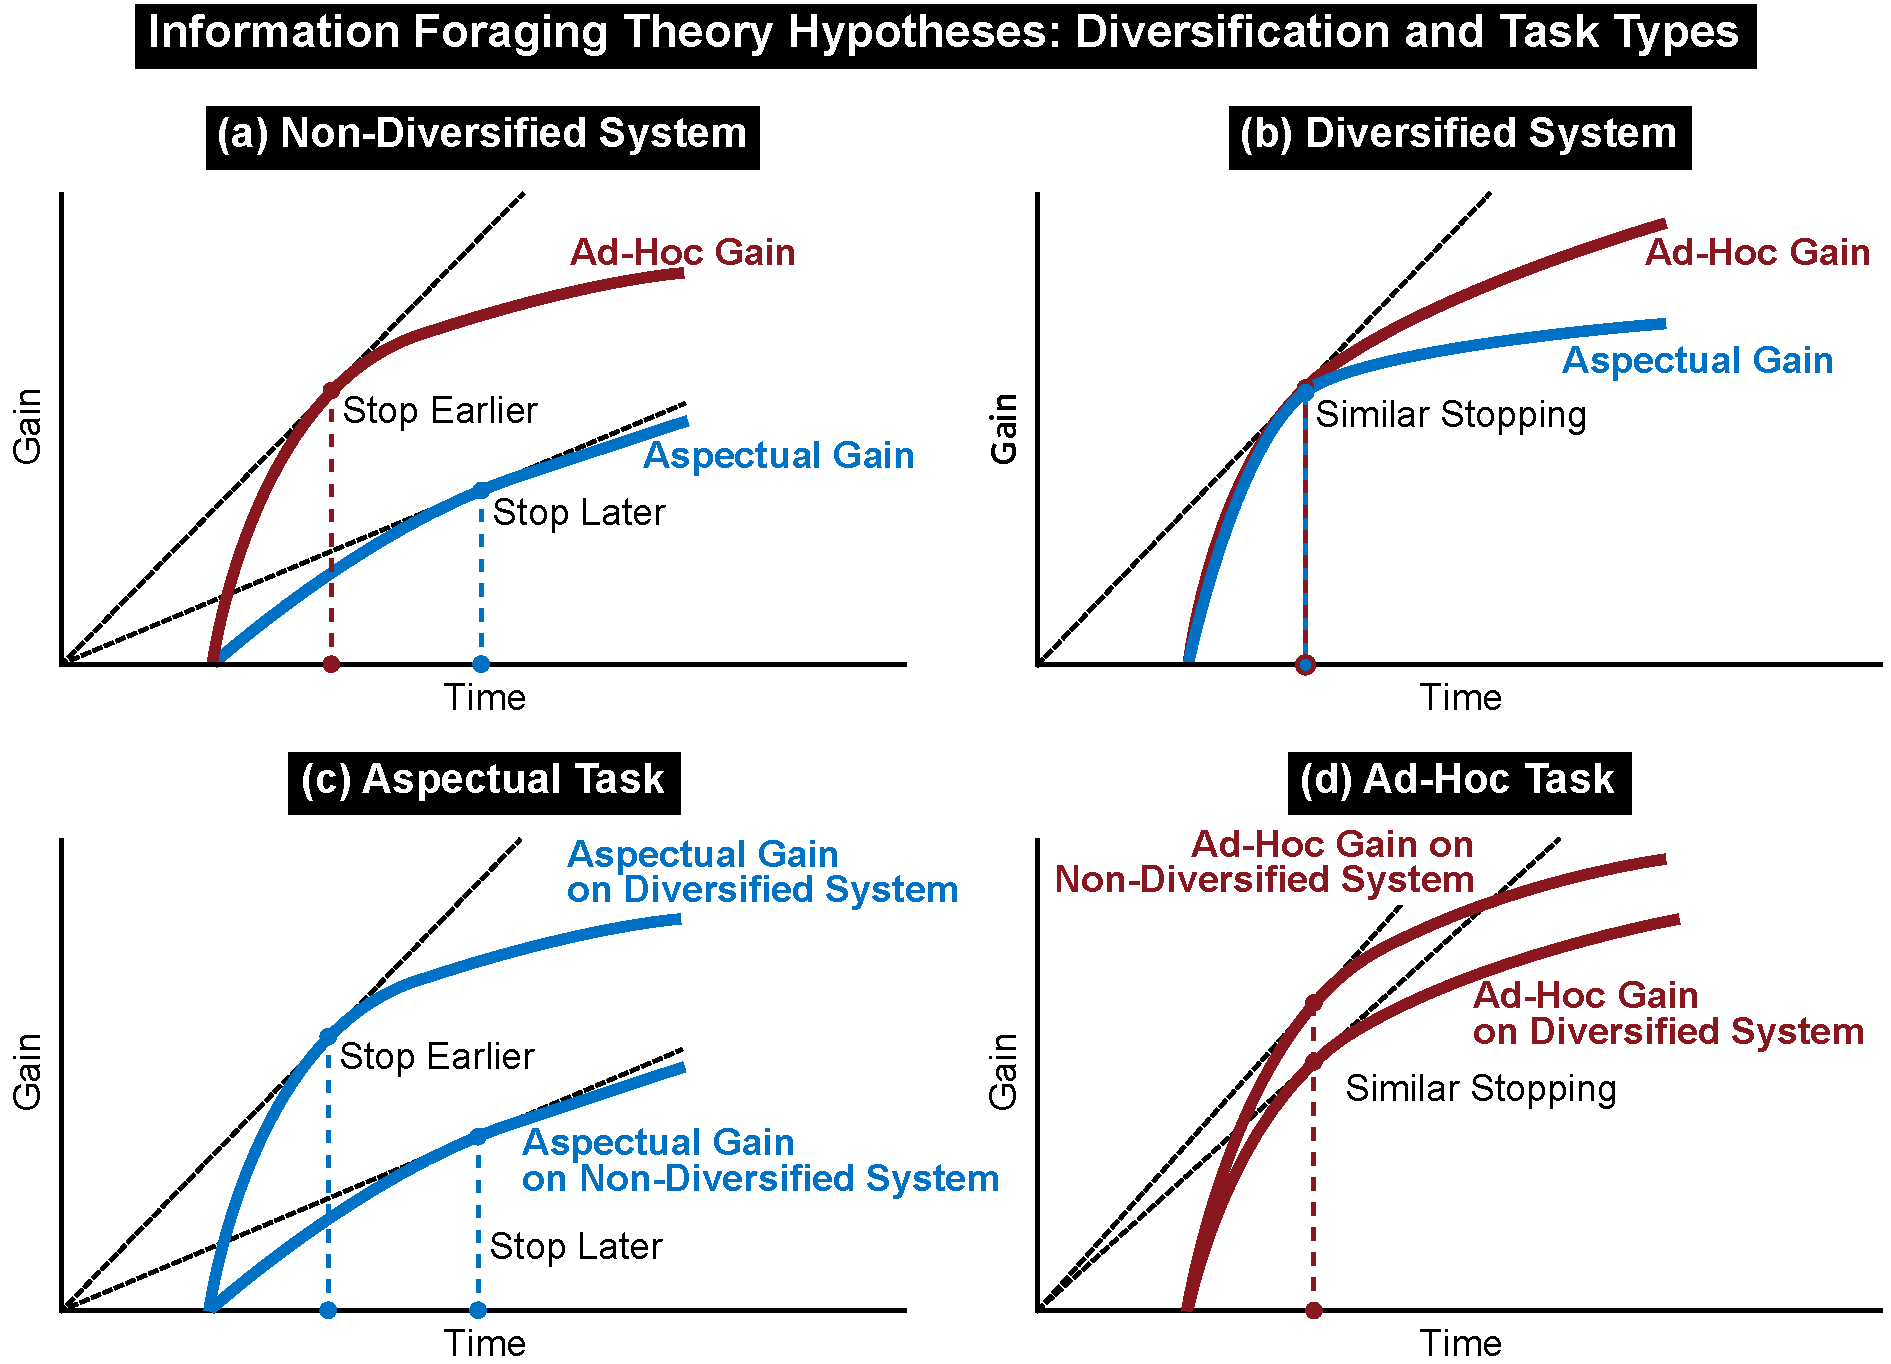
\includegraphics[width=\textwidth]{figures/ift-non-div-fromthesis.pdf}
        \vspace{-2mm}
    \caption{Information Foraging Theory: A graphical depiction of how stopping behaviour is likely to be affected on Diversified System (a), Non-Diversified System (b), Aspectual Task (c) and the Ad-Hoc Task (d).} \label{fig_ift_patches}    
    \vspace{-6mm}
\end{center}
\end{figure}


From IFT, the optimal stopping point would be different between the two tasks. Graphically we can find this point by drawing a line from the origin to the tangent of the gain curve -- the red and blue dots indicating the optimal stopping points for ad-hoc and aspectual retrieval, respectively. Thus, IFT suggests that on the non-diversified system users will examine more documents per query for the aspectual retrieval tasks when compared to the ad-hoc tasks.

In Figure~\ref{fig_ift_patches} (b), where a diversified system is being used, the gain curves for ad-hoc and aspectual retrieval will be similar -- as relevant but different documents are surfaced earlier. In the case of ad hoc topic search, these relevant (even if different) documents will still contribute to the overall gain. And in the case of aspectual retrieval, the relevant and different documents will also contribute to the overall gain -- up to the point where the documents are similar to the previously retrieved material. So IFT seems to suggest that similar stopping behaviours would be observed when searchers use the diversified system. 

Figure~\ref{fig_ift_patches} (c) shows the predicted stopping behaviour for the aspectual task, where we have plotted the aspectual gain curves from the system plots above. Interestingly, IFT suggests that searchers will stop sooner when using the diversified system, and so, if searching for the same amount of time, searchers would thus issue more queries. Finally, Figure~\ref{fig_ift_patches} (d) shows the predicted stopping behaviour for the ad hoc task, where again we have plotted the respective gain curves on each system. Note that the gain curve on the diversity may be a little lower as some irrelevant, but different material may be bubbled up - but as can be seen, we expect little difference between systems, and so the gains, and behaviour, we hypothesise will be approximately the same. Consequently, IFT suggests that there will be little difference regarding stopping behaviours between the systems on the ad-hoc retrieval tasks.

However, we found Information Foraging Theory to go counter to our intuitions on how users will behave. 
When using a standard, non-diversified system, our intuition suggests that since the aspectual retrieval task is rather exploratory, then searchers are more likely to issue more queries as they learn about the topic and try to explore efforts made by different countries to protect different species. In ~\cite{kelly2015search_tasks}, more complex search tasks are shown to require more queries. And if a searcher submits a query that retrieves relevant material such as \texttt{`protecting Pandas in China'}, then we would expect them to only select one or two examples rather than many. In the case of ad hoc topic search, though, we would \emph{intuitively} expect that they would issue fewer queries, and examine more documents - because they don't need to find multiple aspects. However, when using a diversified system, which tries to promote different aspects of the topic, then we would \emph{intuitively} expect that searchers behaviour would change - such that when undertaking aspectual retrieval, they would issue fewer queries, and examine more documents per query. 

\subsection{Research Questions and Hypotheses} \label{sec:questions}
The primary research question of this study is: {\it how does diversification affect the search performance and search behaviour of people when performing ad-hoc topic and aspectual retrieval tasks?} Based on the theoretical analysis above using IFT, we can formulate the specific following hypotheses regarding performance and behaviour:

\begin{itemize}
\item on aspectual retrieval tasks, diversification will lead to:
\begin{description}
\item [H1] fewer documents examined per query, and
\item [H2a] more queries issued, or
\item [H2b] a decrease in task completion time.
\end{description}

\item on ad hoc retrieval tasks, diversification will lead to:
\begin{description}
\item [H3] no difference in the documents examined, and
\item [H4] no difference in the number of queries issued.
\end{description}
\end{itemize}

However, the contradiction between IFT and our intuitions also provides an ulterior hypothesis. Also, given the findings from~\cite{syed2017sal}, we also hypothesise that diversification will lead to a greater awareness of the topic, regardless of the task, and so more aspects will be encountered and found.




%Under IFT, it is assumed that the forager is rational in that (i) they will visit the patch with the highest yield first, and (ii) they wish to maximize their gain per unit of time. To instantiate the model a gain function parameterized by time, i.e., $g(t)$ is required. The point where a forager should move to the next patch is when the maximum gain per unit of time is achieved. This depends on the time it takes to get to a patch, the cost of processing documents, and the distribution of relevant information (as specified by the gain function). 



%!TEX root = jir2018aspects.tex
\section{Experimental Method} \label{sec:method}
To address our research questions and examine the hypotheses as outlined in Section~\ref{sec:questions}, we conducted a within-subjects experiment with two factors: system and task. For the system factor, our baseline control system was based on BM25 (no diversification) and a diversified system based on BM25, re-ranked with xQuAD~\cite{santos2010query_reformulations_diversification}. For the task factor, we used the standard ad-hoc retrieval task and compared against the aspectual retrieval task. This resulted in a $2 \times 2$ factorial design. Therefore, each participant completed four different search tasks, one in each of the four conditions (see below). Conditions were assigned using a Latin square rotation to minimise any ordering effects.

%The corpus, topics and system used closely mirror a prior study undertaken by Maxwell et al.~\cite{maxwell2017snippet_length} in which they examined how the length of result summaries affects search behaviour, performance and experience. Summaries of two snippet fragments (roughly equivalent to two lines) resulted in a good tradeoff in terms of examination time and performance. Labelled interface \textbf{\emph{T2}} in their study, we use two snippet fragments in all experimental conditions, as well as the prior nomenclature in the present study. As such, the four experimental conditions we used in this study are listed below.

\begin{itemize}
\item \textbf{(D.As)} A \textbf{diversified system} with an \textbf{aspectual retrieval} task.
\item \textbf{(ND.As)} A \textbf{non-diversified system} with an \textbf{aspectual retrieval} task.
\item \textbf{(D.Ad)} A \textbf{diversified system} with an \textbf{ad-hoc retrieval} task. 
\item \textbf{(ND.As)} A \textbf{non-diversified system} with an \textbf{ad-hoc retrieval} task.
\end{itemize}

%Further details of the search systems and tasks are provided in Section~\ref{sec:method:systems}. In this section, we also discuss the corpus and topics that were used (Section~\ref{sec:method:corpus}), how we obtained data for aspectual retrieval (Section~\ref{sec:method:entities}), and the diversification algorithm used (Section~\ref{sec:method:diversification}).

%%%%%%%%
\subsection{Corpus and Search Topics}\label{sec:method:corpus}
For this experiment, we used the \emph{TREC AQUAINT} test collection that contains over one million articles from three newswires, collected over the period $1996$-$2000$. The three newswires were: the \emph{Associated Press (AP)}; the \emph{New York Times (NYT)}; and \emph{Xinhua}.  From the TREC 2005 Robust Track~\cite{voorhees2006trec_robust}, we selected five contemporary topics that have been used in prior works~\cite{azzopardi2013query_cost,kelly2009query_suggestion,maxwell2017snippet_length}. These were: 341 \emph{(Airport Security)}; 347 \emph{(Wildlife Extinction)}; 367 \emph{(Piracy)}; 408 \emph{(Tropical Storms)}; and 435 \emph{(Curbing Population Growth)}. These topics were chosen based on evidence from a previous user study with a similar setup, where it was shown that the topics were of similar difficulty and interest~\cite{kelly2009query_suggestion}. Topic~367 was used as a practice topic. The remaining four topics were used as part of the main experimental study.

\subsection{Aspectual and Ad-Hoc Retrieval Tasks}
Participants were asked to imagine that they needed to learn about a number of topics on which they were to write a report on. Given a topic, they were further instructed on whether to focus on finding \emph{relevant} articles in the case of ad-hoc retrieval, or \emph{relevant articles that discussed different aspects} of the topic in the case of aspectual retrieval. For example, for the \emph{Airport Security} topic, participants were required to learn about the efforts taken by international airports to better screen passengers and their carry-on luggage under the ad-hoc retrieval task. For the aspectual retrieval task, they were also asked to find relevant documents that are different and mention \emph{new, previously unseen} airports. Thus, participants were explicitly instructed to find a number of examples from different airports, as opposed to a similar or the same example based in the same airport multiple times.

Participants were instructed to find and save at least four \emph{useful} documents. Depending upon the task being undertaken, \emph{useful} related to a document being either relevant or relevant and different.
%From a previous study, we found it took subjects between 5-10 minutes to save 4-8 relevant documents~\anoncite{maxwell2017snippet_length}.

%%%%%%%%
\subsection{Relevance Judgments and Aspects}\label{sec:method:entities}
For each topic, we used the corresponding TREC QRELs from the TREC 2005 Robust Track to provide the relevance judgements for the study. However, to assess how many aspects were retrieved, we needed to commission additional labels, as existing labels were not available for all the selected topics. For each topic, we first examined the topic descriptions to identify what dimensions could be considered aspects of the topic. We noted that for each topic there were at least two ways this could be achieved: entity- or narrative-based. For example, in the topic \emph{Population Growth}, a document could be relevant if it stated the country (entity-based) or measure that was taken to reduce population growth (narrative-based).
%Thus the country or the measure could be considered different aspects that could be varied, i.e. different countries or different measures or both. 

For this study, it was decided that we should focus on entity-based aspects. This was because \emph{`different narratives'} were subject to greater interpretation than \emph{`different entities'}. For each relevant document, two assessors extracted different aspects, and we found that there were substantially higher agreements (95\% vs 67\%) between assessors across the entity based aspects: (341) airports; (347) species; (367) vessels; (408) storms; and (435) countries; as opposed to the more narrative-based aspects: (341) the security measures taken; (347) the protection and conservation efforts; (367) the acts of piracy; (408) the death and destruction; and (435) the population control methods. Entity-based aspects that we considered for each topic are listed below.

\begin{itemize}
    \item{\textbf{Topic 341 \emph{(Airport Security)}} Different \emph{airports} in which additional security measures were taken, e.g. \emph{John F Kennedy International Airport}, \emph{Boston Logan International Airport}, or \emph{Leonardo Da Vinci International Airport}.}
    \item{\textbf{Topic 347 \emph{(Wildlife Extinction)}} Different \emph{species of endangered animals} under protection by states, e.g. \emph{golden monkey}, \emph{Javan rhino}, or \emph{Manchurian tiger}.}
    \item{\textbf{Topic 367 \emph{(Piracy)}} Different \emph{seaworthy vessels} that were boarded or hijacked, e.g. \emph{Petro Ranger}, \emph{Achille Lauro}, or \emph{Global Mars}.}
    \item{\textbf{Topic 408 \emph{(Tropical Storms)}} Different \emph{tropical storms} where people were killed or there was major damage, e.g. \emph{Hurricane Mitch}, \emph{Typhoon Linda} or \emph{Tropical Storm Frances}.}
    \item{\textbf{Topic 435 \emph{(Curbing Population Growth)}} Different \emph{countries} where population control methods were employed, e.g. \emph{China}, \emph{India} or \emph{Zimbabwe}.}
\end{itemize}

The total number of aspects identified for each topic were: $14$ for 341; $168$ for 347; $18$ for 367; $43$ for 408; and $26$ for 435. Created judgments were saved in the TREC Diversity QREL format, as used by already established evaluation tools that consider aspectual retrieval, such as \texttt{ndeval}\footnote{\url{https://trec.nist.gov/data/web/10/ndeval.c}}.\footnote{In the interests of promoting reproducibility and repeatability, the aspectual judgements created as part of this study are available for download at \url{https://git.io/fpAX8}.} %This, in turn, is used as part of the \emph{TREC Novelty and Diversity Tracks} and  the \emph{TREC 2013 Web Track}~\cite{collinsthompson2013trec}.

%%%%%%%%

\begin{figure}[t!]
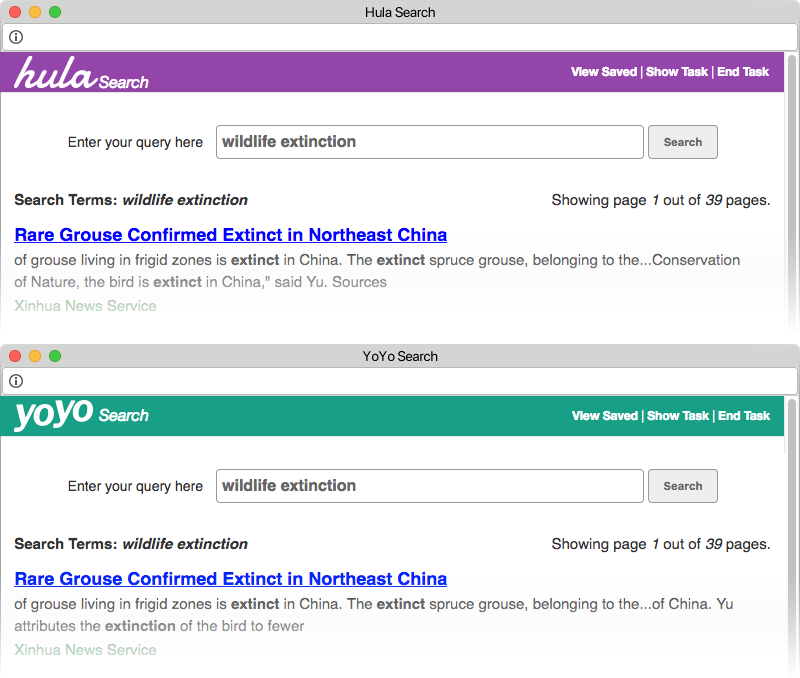
\includegraphics[width=1.0\columnwidth]{figures/interface-both.png}
\caption{The two different retrieval systems and their interfaces, as used in this study. The top screenshot shows \emph{Hula Search} (non-diversified, baseline), with \emph{YoYo Search} (diversified) underneath. Note the different colour schemes that were designed to emphasise the fact that different search systems were being used, without creating too much of a visual distraction.
} 
\label{fig_systems}
\end{figure}

\subsection{Baseline System and User Interfaces}\label{sec:method:systems}
Two experimental search systems were developed. These were identical except regarding branding/logo and the retrieval algorithm used. First, in terms of branding, we created two fictional retrieval system names,
\textbf{\emph{Hula Search}} and \textbf{\emph{YoYo Search}}, for which different colour schemes were devised. The names were chosen as they were not associated with any major retrieval system (to the best of our knowledge), nor did they imply that one of the systems performed better than the other. The colour schemes were chosen to provide the greatest difference in visual appearance to those with colourblindness (two variants of colourblindness, \emph{protanopia} and \emph{deuteranopia}, were both considered). This was to ensure that participants could later indicate which system that they preferred, etc. Screenshots of the two systems in action are provided in Fig.~\ref{fig_systems}. 
Note that a generic \textbf{\emph{NewsSearch}} system -- complete with a blue header -- was used for the practice task. This was to allow participants to familiarise themselves with how to mark and save documents, and how the search functionality worked -- all without becoming favourably or unfavourably biased to one particular system.

For the underlying retrieval system, we used the \emph{Whoosh Information Retrieval (IR)} toolkit.\footnote{Whoosh can be accessed at \texttt{\url{https://pypi.python.org/pypi/Whoosh/}}.} We used BM25 as the retrieval algorithm ($b=0.75$), but with an implicit \texttt{AND}ing of query terms to restrict the set of retrieved documents to only those that contained all query terms provided. This was chosen as most retrieval systems implicitly \texttt{AND} terms together. BM25 served as the baseline control for the non-diversified system condition.

%% Removed table and revised paragraph below to accommodate missing table.
%Table~\ref{tbl:previous_queries} illustrates the parameter sweep when considering the number of new entities found (aspectual recall) within the top $10$ results, re-ranked after applying xQuAD. Similar conclusions could be reached when examining both $\alpha DCG@10$ (where $\alpha=0.5$) and $P@10$. We found that $k=30$ and $\lambda=0.7$ provided the best results in terms of performance and efficiency -- i.e. a higher $k$ only slightly increased performance, but took longer. 

\subsection{Diversifying Results}
For the diversified system, we used BM25 as outlined above to provide the initial ranking and then used xQuAD~\cite{santos2010query_reformulations_diversification} to diversify the ranking. xQuAD has been shown to provide excellent performance for web intent-based diversification. The algorithm used is presented in Alg.~\ref{algo}, complete with a description of the various inputs, the output and helper functions used.

\begin{algorithm}[t!]
\SetAlgoLined
\KwIn{Original ranking, \textit{existingResults}}
\myinput{Diversification depth ($k=30$)}
\myinput{$\lambda=0.7$, weighting for diversification scoring component}
\vspace*{2mm}
\SetKwInput{KwResult}{Output}
\KwResult{Manipulated array of results, diversified to depth $k$}
\vspace*{2mm}
\SetKwInput{KwResult}{Helpers}
\KwResult{\textit{getEntities(x,y,z)} Returns an array results $x$, consisting of entities present in documents in array $x$ from range $y$ to $z$}
\myhelper{\textit{getLength(x)} Returns the length of array $x$}
\myhelper{\textit{getUnseenEntities(x,y)} Returns entities in document $x$ that have not yet}
\myhelper{\hspace*{5mm}been observed in ranked document array $y$}
\myhelper{\textit{sortByScore(x)} Sorts documents array $x$ by \emph{.score} in descending order}
\myhelper{\textit{array.pop()} Removes the top entry from an array, returning its value}
 \vspace*{2mm}
 entities = []\;
 newRankings = []\;
 i = 1\;
 newRankings[0] = existingResults.pop()\;
 
 \While{i $\leq$ k}{
     entities = getEntities(existingResults, 0, i-1)\;
     j = 0\;
     
     \While{j $\leq$ getLength(existingResults)}{
         newEntityCount = getUnseenEntities(document, existingResults)\;
         existingResults[j].score = existingResults[j].score + ($\lambda\cdot$newEntityCount)\;
         j = j + 1\;
     }
     
     sortByScore(existingResults)\;
     newRankings[i] = existingResults.pop()\;
     i = i + 1\;
 }
 \vspace*{3mm}
 \linespread{0.8}
 \caption{\small The algorithm employed to diversify results. Input for this algorithm assumes a ranked list of results, as ranked by the BM25 baseline discussed in the narrative. The diversification algorithm presented is based upon the xQuAD framework~\cite{santos2010query_reformulations_diversification}. Included in the pseudo-code above are a list of input parameters (including the original BM25 ranking) and simple helper functions used within the algorithm.}
 \label{algo}
\end{algorithm}

To select a reasonable approximation for the algorithm's two tuneable input parameters, i.e. $k$ (how many documents to re-rank) and $\lambda$ (how much focus on diversification), we performed a parameter sweep using a set of $715$ training queries from a prior user study~\cite{maxwell2017snippet_length}. Results from this pilot study are presented in Table~\ref{tbl:previous_queries}. As can be seen from the table, we explored a range of $k$ and $\lambda$ values, with $10$--$50$ trialled for $k$, and $0.1$--$1.0$ for $\lambda$. We selected $k=30, \lambda=0.7$ as this configuration provided the best results ($P@10=0.36$, $\alpha DCG@10=0.075$, $AR@10=6.61$, see below for $AR$) in terms of performance and efficiency -- i.e. a higher $k$ only slightly increased performance but took longer to compute.

\begin{table}[t]
    \caption{Table illustrating the effects of varying $\lambda$ and diversifying rank cutoff $k$ using the diversification algorithm as outlined in Alg.~\ref{algo}. Values in the table represent the number of new aspects found (aspectual recall, $AR$) in the top $10$ documents after re-ranking on average, over $715$ queries issued from a prior user study~\cite{maxwell2017snippet_length}. When $\lambda=0.0$, diversification \emph{\textbf{(D)}} is not applied -- this configuration therefore enjoys the same performance as our non-diversified \emph{\textbf{(ND)}}, baseline system that utilises BM25.}
    \label{tbl:previous_queries}
    \renewcommand{\arraystretch}{1.4}
    \begin{center}
    \begin{tabulary}{\textwidth}{L{3.2cm}||D{1.2cm}|D{1.2cm}|D{1.2cm}|D{1.2cm}|D{1.2cm}}
    \hline
    
    % HEADERS
    & \multicolumn{5}{c}{\textbf{Diversification Cutoff (\boldmath{$k$})}} \\
    
    \textbf{Weighting (\boldmath{$\lambda$})} & \boldmath{$10$} & \boldmath{$20$} & \boldmath{$30$} \textbf{\emph{(D)}} & \boldmath{$40$} & \boldmath{$50$} \\ \hline\hline
    
    % VALUES
    % These results came from sigir-2017-combined.csv -- using an Excel PivotTable. No MATLAB script.
    \boldmath{$0.0$} \emph{\textbf{(ND)}} & \multicolumn{5}{c}{$3.64$} \\ \hline
    \boldmath{$0.1$} & $3.64$ & $4.94$ & $5.51$ & $5.95$ & $6.37$ \\ \hline
    \boldmath{$0.3$} & $6.58$ & $6.58$ & $6.64$ & $6.59$ & $6.59$ \\ \hline
    \boldmath{$0.5$} & $6.58$ & $6.58$ & $6.58$ & $5.58$ & $6.58$ \\ \hline
    \boldmath{$0.7$} \emph{\textbf{(D)}} & $6.56$ & $6.56$ & \boldmath{$6.61$} & $6.51$ & $6.60$ \\ \hline
    \boldmath{$0.9$} & $6.52$ & $6.52$ & $6.61$ & $6.57$ & $6.63$ \\ \hline
    \boldmath{$1.0$} & $6.63$ & $6.63$ & $6.59$ & $6.61$ & $6.56$ \\ \hline
    % END
\end{tabulary}
\end{center}
\vspace*{-5mm}
\end{table}

\subsubsection{Aspectual Retrieval Measures}\label{sec_measures}
To measure the performance of the retrieval systems and participants with respect to aspectual retrieval, we utilise two additional measures, reported in tandem with traditional IR measures such as $P@k$. These measures are \emph{Aspectual Recall (AR)} and $\alpha DCG$.

Aspectual recall is defined by Over~\cite{over1998trec} as \emph{``...the fraction of the submitted documents which contain one or more aspects.''} Given a ranking, AR can be computed by summing the number of \emph{unseen, novel aspects} for a topic up to some rank $k$, and dividing by $k$. Therefore, this provides us with a useful means of determining how successful systems and searchers were at identifying documents containing novel aspects.

$\alpha DCG$ also provides us with this ability. An extension of \emph{Discounted Cumulative Gain (DCG)}~\cite{jarvelin2002ndcg}, $\alpha DCG$ employs a position-based searcher model~\cite{clarke2008novelty_diversity} -- similar in nature to its functionally related counterparts, such as $\alpha NDCG$. $\alpha DCG$ takes into account the position at which a document is ranked, along with the aspects contained within the documents. It ranks by rewarding newly-found aspects, and penalising redundant (seen) aspects geometrically, discounting all rewards with a discounting rank function. As the name may imply, $\alpha$ is a tuneable parameter that controls the severity of redundancy penalisation. As used in prior TREC experimentation~\cite{over2001trec}, all values of $\alpha DCG$ reported in this paper are computed with $\alpha=0.5$.

\subsection{Experimental Procedure}
Participants were provided with a link to an online experimental system that first presented the information sheet regarding the experiment. This was then followed by the consent form which participants needed to agree to in order to proceed.\footnote{Ethics approval was sought before the experiment from the Department of Computer and Information Sciences at the University of Strathclyde (ethics approval number 622).} Participants were then asked to fill in a brief demographics survey before undertaking the practice task to familiarise themselves with the interface. Once comfortable with the system, participants could then proceed to undertake the four search tasks. Depending upon the Latin square rotation, participants would then be provided with one of the four conditions on one of the four topics. For each task, participants first completed a pre-task questionnaire. They then moved onto the search task itself. After completion of the task, they were asked to fill in a post-task questionnaire. After completing all four search tasks, participants were then asked to fill in an exit questionnaire regarding which system they preferred. The experiment would then conclude.

%subjects were provided with a traditional search interface -- complete with query box at the top of the interface. Subjects could pose as few or as many queries as they wished, examine result summaries (as can be seen in Figure~\ref{fig_systems}), and \emph{save} documents they thought were relevant and/or contained new aspects. 10 result summaries were presented per \emph{Search Engine Results Page (SERP)}, \`{a} la the \emph{10 blue links}.


%%%%%%%%
\subsection{Recruitment and Controls}\label{sec:method:subjects}
%%%%%%%%
Participants for the experiment were recruited via the crowdsourcing platform \emph{Amazon Mechanical Turk (MTurk)}. Previous work has shown that crowdsourced studies provide similar results as traditional lab-based user studies~\cite{kelly2011remote,zuccon2013crowdsourcing}. However, the caveat here is that this is true only if sufficient controls are in place. If not, workers may attempt to game the system and could, in theory, complete the task poorly~\cite{feild2010turkers}. Therefore, it is important to ensure that quality control mechanisms are in place to mitigate this risk.

First, we ensured that the device being used was desktop-based, and the device's screen resolution was at least $1024 \times 768$ or greater in size. As the experiment was conducted via a web browser (i.e. \emph{Chrome}, \emph{Firefox}, \emph{Safari}, \emph{Edge}, etc.), we wanted to ensure that only the controls provided by the experimental apparatus were used. The experimental system was therefore launched within a popup window of size $1024 \times 768$. Within the popup, all other browser navigation controls (i.e. back buttons, etc.) were disabled (to the best of our abilities). The experimental system was tested on several major (aforementioned) browsers, across a range of different operating systems. This gave us confidence that similar experiences would be had across different systems.

Based upon the suggestions from prior work~\cite{feild2010turkers,zuccon2013crowdsourcing}, workers were only permitted to begin the experiment on the MTurk platform that:

\begin{itemize}
\item were from the United States;
\item were native English speakers;
\item had a \emph{Human Intelligence Task (HIT)} acceptance rate of at least 95\%; and 
\item had at least 100 HITs approved.
\end{itemize}

Requiring the latter two criteria increased the likelihood of recruiting individuals who wanted to maintain their reputation, and would be more likely to complete the study in a satisfactory manner. 

%Subjects were informed that from prior studies~\anoncite{}, that it would take approximately 7-10 minutes to find at least four relevant documents per task - and the duration of the entire experiment would be approximately 40-50 minutes. 
Participants were informed that from our pilot study, it would take approximately 7-10 minutes to find at least four relevant documents per task -- and the duration of the entire experiment would be approximately 40-50 minutes. Since we did not impose any time constraints on how long they searched for, we imposed an accuracy-based control. We informed participants that their accuracy in identifying relevant material would be examined and that they should aim to find four useful documents with at least 50\% accuracy (using the TREC relevance judgments as the gold standard). Note that from a previous lab-based study~\cite{maxwell2017snippet_length} for this set of topics, the accuracy of participants was between 25\% and 40\% on average, depending on the topic. While we stipulated a higher accuracy, this was to motivate participants to work diligently. Since we anticipated the experiment to take just under an hour, participants were compensated with seven dollars (USD).

In all, 64 participants performed the experiment. However, 13 participants were omitted either because they failed to complete all search tasks (five participants were removed), failed to mark at least four documents (two participants were removed), or spent less than two minutes per task and failed to retrieve any relevant documents (six participants were removed). 

Of the 51 participants who successfully completed the experiment, $26$ females and $25$ males participated. The average age of the participants was $38.66$ years ($min=20$; $max=71$; $stdev=11.43$). $22$ of the participants reported having a bachelor's degree or higher, with the remaining $29$ possessing an associate degree or lower. All participants but one expressed \emph{Google} as their everyday retrieval system of choice. All participants indicated that they conducted many searches for information via a retrieval system per week. Nearly three-quarters of the participants (i.e. 38 participants) reported using a mouse for the experiment, with the remaining $13$ using some form of a trackpad.

%Considering the \todo{$32$} participants, and the four sessions each subject undertook, this meant a total of \todo{$128$} search sessions were logged.

%We also implemented a series of log post-processing scripts after completion of the study to further identify and capture individuals who did not perform the tasks as instructed. It was from here that we identified the \todo{$20$} subjects that did not complete the search tasks in a satisfactory way -- attaining an accuracy of less than \todo{$50$\%}. These subjects were excluded from the study, reducing the number of subjects reported from \todo{$40$} to \todo{$32$}.



\subsection{Logging and Measures}\label{sec:method:behaviours}
Below we note the measurements taken while participants used the experimental system.
Our system logged a variety of different events associated with querying and assessing. The generated logs permitted us to measure three different aspects of the search user experience, being: \emph{(i)} interaction; \emph{(ii)} performance; and \emph{(iii)} time. 

\paragraph{Interaction Measures} included the number of queries issued by participants, the number of documents that were examined, the number of different SERPs viewed, and the depths to which participants clicked on (and hovered over) result summaries. It should be noted that components recorded such as hover depths over result summaries were inferred from the movement of the mouse cursor -- eye-tracking equipment was not used in this study. In prior studies, the position of the mouse cursor on the screen has correlated strongly with the user's gaze on the screen~\cite{chen2001mouse_cursor,smucker2014judging_relevance_movements}.
\vspace*{2mm}

\paragraph{Performance Measures} included the number of documents that were saved by participants, denoting that they were either relevant (for ad-hoc retrieval), or relevant and contained new information (for aspectual retrieval). From this, we could also break this number down into the number of documents that were saved and TREC relevant -- as well as TREC non-relevant -- and $P@k$ measures at varying depths for the performance of the queries issued by the participants. Using the diversity QRELs (generated as per the description in Section~\ref{sec:method:entities}), we were able to determine how well the query performed with respect to how many new entities were in the top $k$ results, and the $\alpha$DCG scores for each query. In addition, using the list of saved documents, we could also then identify how many entities that participants had found, and how many documents contained one or more unseen entities -- both in terms of the context of results of the current query, and the overall search session (over all the queries issued).

From the log data, we could also compute additional performance measures such as the accuracy that searchers reached during each session, as well as the \emph{probabilities of interaction.} In the context of this study, accuracy referred to the ratio of documents that were TREC relevant, versus the total numbers of documents saved. For example, if a searcher saved four documents during a search session, with three of them being TREC relevant, the searcher's accuracy was $3/4 = 0.75$. The interaction probabilities that we considered included: the probabilities of clicking on a result summary link ($P(C)$) -- given that it was either TREC relevant ($P(C|R)$) or TREC non-relevant ($P(C|N)$), and the probabilities of marking a document that was clicked ($P(M)$) -- again, given that it was either TREC relevant ($P(M|R)$) or TREC non-relevant ($P(M|N)$).

\paragraph{Time-Based measures} included the time spent issuing queries (from query focus to issuance), the time spent on a SERP -- as well as examining result summaries\footnote{Result summary times were approximated by dividing the total recorded SERP time by the number of snippets hovered over with the mouse cursor. We believe this is a reasonable assumption to make -- network latency issues beyond our control meant that mouse hover events occasionally were delivered at the wrong times, and as such were logged in the incorrect order.} -- and the time spent examining documents. These times could then allow us to compute the total amount of time spent during the session.

%%%%%%%%
\subsection{User Experience}\label{sec:method:experience}
%%%%%%%%
To capture their perceived experiences, we asked participants to complete both pre- and post-task surveys for each of the four experimental conditions that they were presented with during the experiment.

Pre-task surveys consisted of five questions, each of which was on a seven-point Likert scale ($1$ -- strongly disagree to $7$ -- strongly agree). Participants were sought for their opinions on their: \emph{(i)} prior knowledge of the topic; \emph{(ii)} the relevancy of the topic to their lives; \emph{(iii)} their desire to learn about the topic; \emph{(iv)} whether they had searched on this topic before; and \emph{(v)} the perceived difficulty to search for information on the topic.

Following the completion of each search task, participants were provided with a post-task survey, again using a seven-point Likert scale for responses. The survey considered aspects of \emph{(i)} their behaviour, and \emph{(ii)} how they felt the system performed. Considering their behaviours, participants were asked for their opinions on:

\begin{itemize}
\item how successful they thought they were at completing the task \emph{\textbf{(success)}}; 
\item how quickly they felt they completed the task \emph{\textbf{(participant speed)}}; 
\item whether they issued different queries to explore the topic \emph{\textbf{(queries)}}; 
\item if they only examined a few documents per query \emph{\textbf{(documents)}}; 
\item whether they checked each document carefully before saving \emph{\textbf{(checks)}}; and 
\item whether they saved more documents than was required, with a minimum of four being required \emph{\textbf{(more)}}. 
\end{itemize}
Participants were also asked for their opinions on: 
\begin{itemize}
\item whether they thought the system helped them complete the task quickly \emph{\textbf{(system speed)}}; 
\item whether they felt the system made it difficult to find useful information \emph{\textbf{(difficulty)}}; 
\item if the system made it easy to complete the task \emph{\textbf{(ease)}}; 
\item if they were happy with how the system performed \emph{\textbf{(happiness)}}; 
\item whether the system was cumbersome or not \emph{\textbf{(cumbersome)}}; and 
\item whether they were confident in the decisions they made \emph{\textbf{(confident)}}. 
\end{itemize}

Upon completion of the experiment, participants were provided with an exit survey consisting of several questions. Here, we wanted to ascertain which of the two search system offered the best performance, and which one they preferred. Answers were provided on a scale this time from $1-6$, with: $1$ denoting \emph{definitely Hula Search} (non-diversified); $3$ denoting \emph{slightly Hula Search;} $4$ denoting \emph{slightly YoYo Search}; and $6$ denoting \emph{definitely YoYo Search} (diversified). We opted not to include a neutral position to force participants into deciding between one of the two systems. We asked participants:

\begin{itemize}
    \item{which system was most informative \emph{\textbf{(informative)}};}
    \item{which system was more unhelpful \emph{\textbf{(unhelpful)}};}
    \item{what one was easier to use \emph{\textbf{(easiest)}};}
    \item{what system was less useful \emph{\textbf{(least useful)}};}
    \item{what system returned more relevant information \emph{\textbf{(most relevant)}};}
    \item{what system offered a more diverse set of results \emph{\textbf{(most diverse)}}; and}
    \item{what system they preferred overall \emph{\textbf{(most preferable)}}.}
\end{itemize}

%We provided a scale from $1$-$6$, from $1$ (definitely \emph{Diversified System Name}) to $3$ (slightly \emph{Diversified System Name}), from $4$ (slightly \emph{Non-Diversified System Name}) to $6$ (definitely \emph{Non-Diversified System Name}). We opted not to include a neutral option to force the subjects into deciding between one of the two systems. We asked subjects: which system was most informative \emph{\textbf{(informative)}}; which was the most unhelpful \emph{\textbf{(unhelpful)}}; which was easiest \emph{\textbf{(easiest)}}; which was the most useful \emph{\textbf{(useful)}}; which system returned the most \emph{relevant} information \emph{\textbf{(rel. preferred)}}; which system returned the most \emph{diverse} information \emph{\textbf{(div. preferred)}}; and which system was preferred overall \emph{\textbf{(preferred)}}.

% From results; moved here to fit in the correct place in the paper.
\begin{table}[t]
    \caption{Query statistics and performance measures across both of the experimental systems trialled, \textbf{\textit{ND}} (Non-Diversified) and \textbf{\textit{D}} (Diversified). Note the significant differences between the diversity-centric measures, \boldmath{$\alpha DCG$} (where \boldmath{$\alpha=0.5$}) and aspectual recall (\boldmath{$AR$}), highlighting that the diversification algorithm did indeed provide a more diverse set of results to the participants.}
    \label{tbl_queryperf_2018}
    \renewcommand{\arraystretch}{1.5}
    \begin{center}
    \begin{tabulary}{\textwidth}{L{0.2cm}L{5.75cm}|D{2.1cm}|D{2.1cm}}
    %\begin{tabulary}{\textwidth}{cc|c|c}
    
    \hline
    
    % OUTPUT FROM script
    &  & \textbf{\emph{ND}} & \textbf{\emph{D}} \\ \hline\hline
    & \textbf{\emph{Queries Issued}} & $718$ & $555$ \\ \hline
    & \textbf{\emph{Terms per Query}} & $3.59$ & $3.80$ \\ \hline
    & \textbf{\emph{Unique Terms}} & $345$ & $292$ \\ \hline\hline
     
    \multirow{2}{*}{\rotatebox{90}{\hspace*{-1mm}\small{\boldmath{$Prec.$}}}} & \boldmath{$P@5$} & $0.25\pm 0.01$* & $0.29\pm 0.01$*  \\ \cline{2-4}
    & \boldmath{$P@10$} & $0.22\pm 0.01$ & $0.24\pm 0.01$  \\ \hline\hline
      
    \multirow{2}{*}{\rotatebox{90}{\hspace*{-1mm}\small{\boldmath{$\alpha DCG$}}}} & \boldmath{$\alpha DCG@5$} & $0.02\pm 0.00$* & $0.04\pm 0.00$* \\ \cline{2-4}
    & \boldmath{$\alpha DCG@10$} & $0.03\pm 0.00$* & $0.04\pm 0.00$* \\ \hline\hline
       
    \multirow{2}{*}{\rotatebox{90}{\hspace*{-1mm}\small{\boldmath{$AR$}}}} & \boldmath{$AR@5$} & $1.40\pm 0.11$* & $3.39\pm 0.21$*  \\ \cline{2-4}
    & \boldmath{$AR@10$} & $2.11\pm 0.14$* & $4.07\pm 0.24$*  \\ \hline    
    \end{tabulary}
    \vspace*{-4mm}
    \end{center}
\end{table}


%!TEX root = jir2018aspects.tex
\begin{table}
 \centering
    \caption{Behavioural and performance measures reported across the four experimental conditions (top table), systems and tasks (bottom table).}
    \label{tbl_actions}
    \renewcommand{\arraystretch}{1.4}
    %\begin{center}
    %\begin{small}
    \begin{tabulary}{\textwidth}{L{3.4cm}||D{1.55cm}|D{1.55cm}|D{1.55cm}|D{1.55cm}}
    %\begin{tabulary}{\textwidth}{|c||c|c|c|c|}
    \hline
    % OUTPUT FROM script
    & \multicolumn{4}{c}{\textbf{Experimental Conditions}} \\
    \cline{2-5}
    \textbf{Actions} & \textbf{\emph{D.As}} & \textbf{\emph{ND.As}} & \textbf{\emph{D.Ad}} & \textbf{\emph{ND.Ad}}\\  \hline\hline
    % START DATA
    \textbf{\emph{\#Queries}} & 5.92$\pm$ 0.88 & 5.25$\pm$ 0.80 & 4.96$\pm$ 0.74 & 5.20$\pm$ 0.69 \\ \hline
    \textbf{\emph{\#SERPs/Query}} & 1.78$\pm$ 0.14 & 2.42$\pm$ 0.24 & 2.28$\pm$ 0.31 & 2.28$\pm$ 0.20 \\ \hline
    \textbf{\emph{Documents/Query}} & 3.02$\pm$ 0.39 & 3.65$\pm$ 0.46 & 3.48$\pm$ 0.51 & 3.23$\pm$ 0.37 \\ \hline
    \textbf{\emph{Depth/Query}} & 12.85$\pm$ 1.49 & 15.73$\pm$ 1.45 & 16.19$\pm$ 2.14 & 13.94$\pm$ 1.93 \\ \hline\hline
    \textbf{\emph{\#Saved}} & 5.80$\pm$ 0.26 & 5.96$\pm$ 0.25 & 5.92$\pm$ 0.25 & 5.78$\pm$ 0.20 \\ \hline
    \textbf{\emph{\#TREC Saved}} & 2.63$\pm$ 0.22 & 2.18$\pm$ 0.23 & 2.51$\pm$ 0.23 & 2.22$\pm$ 0.22 \\ \hline
    \textbf{\emph{\#TREC Non-Relevant}} & 1.75$\pm$ 0.22 & 1.96$\pm$ 0.23 & 1.37$\pm$ 0.22 & 1.82$\pm$ 0.23  \\ \hline
    \textbf{\emph{\#Entities Found}} & 7.22$\pm$ 0.94* & 4.31$\pm$ 0.60* & 5.82$\pm$ 0.77 & 4.37$\pm$ 0.59*  \\ \hline
    \textbf{\emph{\#Docs w/ New Entities}} & 3.20$\pm$ 0.21* & 2.35$\pm$ 0.20* & 2.63$\pm$ 0.23 & 2.02$\pm$ 0.18* \\ \hline
    \end{tabulary}
    
    \vspace{5mm}
    
    \begin{tabulary}{\textwidth}{L{3.4cm}||D{1.55cm}|D{1.55cm}|D{1.55cm}|D{1.55cm}}
    %\begin{tabulary}{\textwidth}{|c||c|c|c|c|}
    \hline
         & \multicolumn{2}{c|}{\textbf{Systems}} & \multicolumn{2}{c}{\textbf{Tasks}} \\
         \cline{2-5}
 \textbf{Actions}       & \textbf{\emph{ND}} & \textbf{\emph{D}} & \textbf{\emph{Ad.}} & \textbf{\emph{As.}} \\
        \hline
        \hline
 \textbf{\emph{\#Queries}} & 5.23$\pm$ 0.53 & 5.44$\pm$ 0.58 & 5.08$\pm$ 0.51 & 5.59$\pm$ 0.59 \\ \hline
 \textbf{\emph{\#SERPs/Query}} & 2.35$\pm$ 0.16 & 2.03$\pm$ 0.17 & 2.28$\pm$ 0.18 & 2.10$\pm$ 0.14 \\ \hline
 \textbf{\emph{Documents/Query}} & 3.44$\pm$ 0.29 & 3.25$\pm$ 0.32 & 3.36$\pm$ 0.31 & 3.34$\pm$ 0.30 \\ \hline
 \textbf{\emph{Depth/Query}} & 14.84$\pm$ 1.58 & 14.52$\pm$ 1.31 & 15.07$\pm$ 1.44 & 14.29$\pm$ 1.47 \\ \hline\hline
 \textbf{\emph{\#Saved}} & 5.87$\pm$ 0.16 & 5.86$\pm$ 0.18 & 5.85$\pm$ 0.16 & 5.88$\pm$ 0.18 \\ \hline
 \textbf{\emph{\#TREC Saved}}  & 2.20$\pm$ 0.16 & 2.57$\pm$ 0.16 & 2.36$\pm$ 0.16 & 2.40$\pm$ 0.16 \\ \hline
    \textbf{\emph{\#TREC Non-Relevant}}  & 1.89$\pm$ 0.16 & 1.56$\pm$ 0.16 & 1.60$\pm$ 0.16 & 1.85$\pm$ 0.16 \\ \hline
    \textbf{\emph{\#Entities Found}}  & 4.34$\pm$ 0.42* & 6.52$\pm$ 0.61* & 5.10$\pm$ 0.49 & 5.76$\pm$ 0.57 \\ \hline
    \textbf{\emph{\#Docs w/ New Entities}} & 2.19$\pm$ 0.13* & 2.91$\pm$ 0.16* & 2.32$\pm$ 0.15* & 2.77$\pm$ 0.15* \\ \hline     

       % END DATA
    \end{tabulary}
    %\end{small}
    %\end{center}
\end{table}


\begin{table}
%\begin{table*}[t]
    \caption{Interaction times across each experimental condition (top table), system and task (bottom table). Included is: the mean total session time \emph{(Total Session)}; the per query time \emph{(Per Query)}; the per document time \emph{(Per Document)}; and the per result summary (snippet) time \emph{(Per Snippet)}. Also included are mean total times. Results are presented in seconds.}
    \label{tbl_times}
    \renewcommand{\arraystretch}{1.4}
    \begin{center}
         \begin{tabulary}{\textwidth}{L{2.05cm}||D{1.9cm}|D{1.9cm}|D{1.9cm}|D{1.9cm}}
    \hline   
   % OUTPUT FROM script
    & \multicolumn{4}{c}{\textbf{Experimental Conditions}}  \\
    \cline{2-5}
    \textbf{Time} & \textbf{\emph{D.As}} & \textbf{\emph{ND.As}} & \textbf{\emph{D.Ad}} & \textbf{\emph{ND.Ad}}  \\ \hline\hline
    
\textbf{\emph{Total Session}} & \small{443.65$\pm$ 45.05} & \small{430.50$\pm$ 38.39} & \small{432.18$\pm$ 49.87} & \small{447.55$\pm$ 47.82}  \\ \hline\hline
\textbf{\emph{Total Query}} & \small{45.26$\pm$ 6.48} & \small{47.76$\pm$ 8.41} & \small{46.40$\pm$ 8.01} & \small{43.22$\pm$ 6.55} \\ \hline
\textbf{\emph{Per Query}} & \small{8.80$\pm$ 0.89} & \small{9.99$\pm$ 1.21} & \small{9.69$\pm$ 0.79} & \small{8.69$\pm$ 0.57} \\ \hline\hline
\textbf{\emph{Total Doc.}} & \small{162.93$\pm$ 20.47} & \small{144.85$\pm$ 16.73} & \small{139.58$\pm$ 16.70} & \small{152.83$\pm$ 27.69} \\ \hline
\textbf{\emph{Per Document}} & \small{15.97$\pm$ 1.96} & \small{13.03$\pm$ 1.01} & \small{13.66$\pm$ 1.02} & \small{15.09$\pm$ 2.20}  \\ \hline\hline
\textbf{\emph{Per Snippet}} & \small{1.59$\pm$ 0.09} & \small{1.75$\pm$ 0.15} & \small{1.71$\pm$ 0.11} & \small{1.71$\pm$ 0.13} \\ \hline

    \end{tabulary}
    
    \vspace{5mm}
    
    \begin{tabulary}{\textwidth}{L{2.05cm}||D{1.9cm}|D{1.9cm}|D{1.9cm}|D{1.9cm}}
        \hline

& \multicolumn{2}{c|}{\textbf{Systems}} & \multicolumn{2}{c}{\textbf{Tasks}} \\
 \cline{2-5}
\textbf{Time} & \textbf{\emph{ND}} & \textbf{\emph{D}} & \textbf{\emph{Ad.}} & \textbf{\emph{As.}} \\ \hline\hline
\textbf{\emph{Total Session}} & \small{439.02$\pm$ 30.52} & \small{437.91$\pm$ 33.44} & \small{439.86$\pm$ 34.38} & \small{437.08$\pm$ 29.45} \\ \hline\hline
\textbf{\emph{Total Query}} & \small{45.49$\pm$ 5.31} & \small{45.83$\pm$ 5.13} & \small{44.81$\pm$ 5.15} & \small{46.51$\pm$ 5.28} \\ \hline
\textbf{\emph{Per Query}}  & \small{9.34$\pm$ 0.67} & \small{9.25$\pm$ 0.59} & \small{9.19$\pm$ 0.49} & \small{9.39$\pm$ 0.75} \\ \hline\hline
\textbf{\emph{Total Doc.}} & \small{148.84$\pm$ 16.10} & \small{151.26$\pm$ 13.19} & \small{146.21$\pm$ 16.10} & \small{153.89$\pm$ 13.18} \\ \hline
\textbf{\emph{Per Document}}  & \small{14.06$\pm$ 1.21} & \small{14.81$\pm$ 1.10} & \small{14.37$\pm$ 1.21} & \small{14.50$\pm$ 1.11} \\ \hline\hline
\textbf{\emph{Per Snippet}} & \small{1.73$\pm$ 0.10} & \small{1.65$\pm$ 0.07} & \small{1.71$\pm$ 0.08} & \small{1.67$\pm$ 0.09} \\ \hline
    % END OUTPUT
    \end{tabulary}
    \end{center}
%\end{table*}
\end{table}







%%%%%%%%%%%%%%%%%%%%%%%%%%%%%%%%%%%%%%%%%%%%%%%%%%%%%%%%%%%%%%%%%%%%%%%%%%%
\section{Results} \label{sec:results}
%%%%%%%%%%%%%%%%%%%%%%%%%%%%%%%%%%%%%%%%%%%%%%%%%%%%%%%%%%%%%%%%%%%%%%%%%%%

We now address our research questions and hypotheses as addressed in Section~\ref{sec:questions}. Both the behaviour and performance of each subject were analysed across each of the four experimental conditions, \textbf{\emph{D.As}}, \textbf{\emph{ND.As}}, \textbf{\emph{D.Ad}} and \textbf{\emph{ND.Ad}}. Task (\emph{\textbf{As}}. vs \emph{\textbf{Ad.}}) and System (\emph{\textbf{ND.}} vs \emph{\textbf{D.}}) effects were also examined. To evaluate these data, ANOVAs were conducted using the conditions, systems and tasks each as factors; main effects were examined with $\alpha=0.05$. Bonferroni tests were then used for post-hoc analysis. It should be noted, however, that where $\alpha DCG$ is reported, we compute the values using $\alpha=0.5$.

To begin with our analysis, we first examined whether the performance experienced by participants on the two systems was, in fact, different (as indicated by our pilot study). We took the queries participants issued to each system and measured the performance according to $\alpha DCG$, aspectual recall and precision (see Table~\ref{tbl_queryperf_2018}). Statistical testing confirms that the two systems were significantly different 
 in terms of diversity (i.e. $\alpha DCG@10$: $F(1, 1272=28.74, p<0.001)$, and apectual recall$@10$: $F(1, 1272=55.43, p<0.001)$). However, $P@10$ was not significantly different - suggesting that the re-ranking promoted relevant and diverse documents, but only in the top 10 on average.
 
 Aside from showing query performance, Table~\ref{tbl_queryperf_2018} also reports the number of terms issued per query over each systems \textbf{\emph{ND}} and \textbf{\emph{D}}; of the $1273$ queries issued, those issued to \textbf{\emph{ND}} were shorter on average, with $3.59$ terms compared to $3.80$ terms for \textbf{\emph{D}}. However, the vocabulary used by subjects issuing queries to \textbf{\emph{ND}} was greater than \textbf{\emph{D}} -- queries issued to \textbf{\emph{ND}} contained $345$ unique terms, compared to $292$ for \textbf{\emph{D}}.
This provides our first finding of note. When using \textbf{\emph{ND}}, participants issued more queries -- but were slightly shorter and more varied -- to accomplish their tasks. 


\begin{table}[t!]
    \caption{Interaction probabilities, as observed over the four experimental conditions trialled in this study. Refer to Section~\ref{sec:method:behaviours} for an explanation of each probability's meaning.}
    \label{tbl_probabilities}
    \renewcommand{\arraystretch}{1.4}
    \begin{center}
    \begin{small}
    \begin{tabulary}{\textwidth}{L{3.2cm}||D{1.6cm}|D{1.6cm}|D{1.6cm}|D{1.6cm}}
   
   \hline
    
    % OUTPUT FROM script
    \textbf{Probability} & \textbf{\emph{D.As}} & \textbf{\emph{ND.As}} & \textbf{\emph{D.Ad}} & \textbf{\emph{ND.Ad}} \\ \hline\hline
    \boldmath{$P(C)$} & 0.16$\pm$ 0.01* & 0.21$\pm$ 0.02* & 0.16$\pm$ 0.01* & 0.20$\pm$ 0.01* \\ \hline
    \boldmath{$P(C|R)$} & 0.27$\pm$ 0.03 & 0.30$\pm$ 0.04 & 0.25$\pm$ 0.03 & 0.31$\pm$ 0.04 \\ \hline
    \boldmath{$P(C|N)$} & 0.13$\pm$ 0.02* & 0.18$\pm$ 0.02* & 0.13$\pm$ 0.01* & 0.17$\pm$ 0.02* \\ \hline\hline
    \boldmath{$P(M)$} & 0.67$\pm$ 0.03 & 0.66$\pm$ 0.03 & 0.70$\pm$ 0.03 & 0.71$\pm$ 0.04 \\ \hline
    \boldmath{$P(M|R)$} & 0.78$\pm$ 0.04 & 0.63$\pm$ 0.05 & 0.74$\pm$ 0.04 & 0.67$\pm$ 0.05 \\ \hline
    \boldmath{$P(M|N)$} & 0.59$\pm$ 0.04 & 0.61$\pm$ 0.04 & 0.65$\pm$ 0.04 & 0.65$\pm$ 0.04 \\ \hline
    % END REDUCED OUTPUT
    \end{tabulary}
    \end{small}
    \end{center}
\end{table}

%%%%%%%%%%%%%%%
\subsection{Observed Behaviours}
%%%%%%%%%%%%%%%
\paragraph{Interactions.} Table~\ref{tbl_actions} presents the mean (and standard deviations) of \textit{(i)} the number of queries issued, \textit{(ii)} the number of SERPs that were examined by subjects per query, \textit{(iii)} the number of documents examined (clicked) per query, and \textit{(iv)} the click depth (or search stopping depth) per query. %These mean values are compared in three ways: \emph{(i)} over each of the four experimental conditions trialled; \emph{(ii)} over the two experimental systems (non-diverse vs. diverse) and \emph{(iii)} over the two different search tasks (ad-hoc vs. aspectual). 
Statistical tests reveal no effects across conditions, systems or tasks. However, there are several trends that are worth mentioning. Firstly, we notice that when participants used the diversified system to complete the aspectual retrieval task, they examined fewer documents per query than when completing the same task on the non-diversified system (12.85 vs. 15.73) -- which is in line with \emph{H1}. We also observed that participants issued slightly more queries on the diversified system compared to the non-diversified system with the aspectual retrieval task (5.92 vs. 5.25) -- which is in line with \emph{H2a} --- but these results were not significantly significant.

%Considering a diversified system, an aspectual retrieval topic, as outlined by \emph{H1}, result in fewer documents examined per query. Evidence shown in Table~\ref{tbl_post_behavioural} suggests that this may hold, with $3.02\pm0.39$ documents per query examined under \textbf{\emph{D.As}}, compared to a slightly larger number of $3.65\pm0.46$ documents per query for the non-diversified equivalent, \textbf{\emph{ND.As}}.

%IFT suggests that if a lower number of documents are examined per query, then the number of queries, over a similar task completion time, will increase, leading to hypotheses \emph{H2a} and \emph{H2b}. Looking again at Table~\ref{tbl_post_behavioural}, this holds -- \textbf{\emph{D.As}} sees $5.92\pm0.88$ queries issued, compared to the non-diversified equivalent, \textbf{\emph{ND.As}}, reaching a lower value of $5.25\pm0.80$.

Turning our attention to the ad-hoc retrieval tasks, while our hypotheses suggested that there would be no differences in terms of the number of documents examined \emph{(H3)} or in the number of queries issued \emph{(H4)} -- which was the case -- however we note that participants on the diversity system inspected more results than when on the non-diversified system (16.19 vs. 13.94), and they issued slightly fewer queries (4.96 vs 5.20). We can see the trade-offs between queries and the number of results inspected per query, where more queries tend to lead to fewer results being examined, and vice versa. This trend suggests that participants, when searching on the diversified system, for relevance, may have had to dig deeper, to find more relevant material (due to system performance), or that the system encouraged participants to go deeper (which is what we intuitively inspected when they were searching for diversity). Either way, we find no conclusive evidence to support the studies main hypotheses -- only trends. 

Table~\ref{tbl_probabilities} reports interaction probabilities associated with user interactions, i.e. the probability of marking a document saved $P(M)$, and the probability of clicking a document $P(C)$ along with the conditional probabilities for each based on whether the document saved or clicked was TREC (R)elevant or (N)on-Relevant. From the table, we can see that there was a significant difference between conditions (and systems, not shown) for the probability of a click, and the probability of clicking on non-relevant items. Comparing systems indicated that participants clicked more when using the non-diversified system, and clicked on more non-relevant documents. However, we did not observe any task effects. This suggests that the non-diversified system affected led to examining more documents, but often more non-relevant documents. This is reflected by the fact that across all the performance measures (see below), participants on the non-diversified system performed worse.

%%%%%%%%%%%%%%%
\paragraph{Time-Based Measures.} Table~\ref{tbl_times} reports the time taken for various interactions, across each condition, system and task. We report: the mean total session time (from the first query focus to ending the task); the mean time spent entering queries; the mean per document examination time; and the mean time spent examining a result summary (or snippet). All values are reported in seconds. Surprisingly, no significant differences were found between any of the comparisons over the total session times, the per query times, the per document times, and the per snippet times. Results, however, do show a relatively constant mean session time over each of the four experimental conditions, at $\approx438.5$ seconds, which is about $7$ minutes, on average -- this was in line with the time taken to find four documents in our previous studies with similar workers~\anoncite{\cite{maxwell2017snippet_length}} and lab participants~\anoncite{\cite{maxwell2016agents}}.
Considering hypothesis \emph{H2b}, no evidence was found to support that under the diversity system \textbf{\emph{D}} with an aspectual task that completion times would be lower. Here, we can see that they were in fact slightly higher (443 seconds \textbf{\emph{D}} vs. 430 seconds on \textbf{\emph{ND}}, i.e. the difference of about examining one more document). 

%%%%%%%%%%%%%%%
\paragraph{Performance.} In Table~\ref{tbl_actions}, we also report a number of performance measures: the number of saved documents -- also broken down into the number of TREC saved and TREC non-relevant and saved, along with the number of new entities found (within saved documents, with new being in the context of a search session) -- and the number of documents containing at least one new entity. In terms of the documents saved, there were no significant differences between conditions, systems or tasks. On average, participants saved around six documents on average, which was two more than the goal set, $4$ -- suggesting that wanted to make sure that they found a few extra, just in case some were not relevant/useful.

However, when we look at the entity-related measures, we note that participants found more documents that contained new entities and found more entities overall when using the diversity system. This was significantly different ($6.52\pm0.61$ compared to $4.34\pm0.42$ respectively, where $F(1, 203=8.70, p<0.05)$). When examining each condition, the Bonferroni follow-up test showed significant differences were observed between condition \textbf{\emph{D.As}} and conditions \textbf{\emph{D.Ad}} and \textbf{\emph{ND.Ad}}, where $F(3, 203=3.49, p<0.05)$. Also, we notice that participants also found more documents with entities, and more entities when using the ad-hoc retrieval task when using the diversity system than when they used the non-diversity system (docs with entities: 2.63 vs. 2.02, new entities: 5.82 vs 4.37). Though this was not significantly different, it does suggest that when participants used the diversity system, they did learn more about the different aspects of the topic (or at least encountered more aspects) than when using the non-diversity system. 

\paragraph{Post Task and Post System Questionnaires.} There were no notable significant differences between conditions, tasks, or system for any of the post-task questions. For the post system questionnaires, participants were roughly evenly split between their preference for the diversified or non-diversified system -- again with no significant differences. This finding suggests that despite the substantial (and significant) difference in aspectual recall and other system performance measures, between the systems, participants seemed largely ambivalent to the different system's influence. Though, of course, their observed behaviours do suggest that the system (and task) did affect their performance.

\begin{figure}[t!]
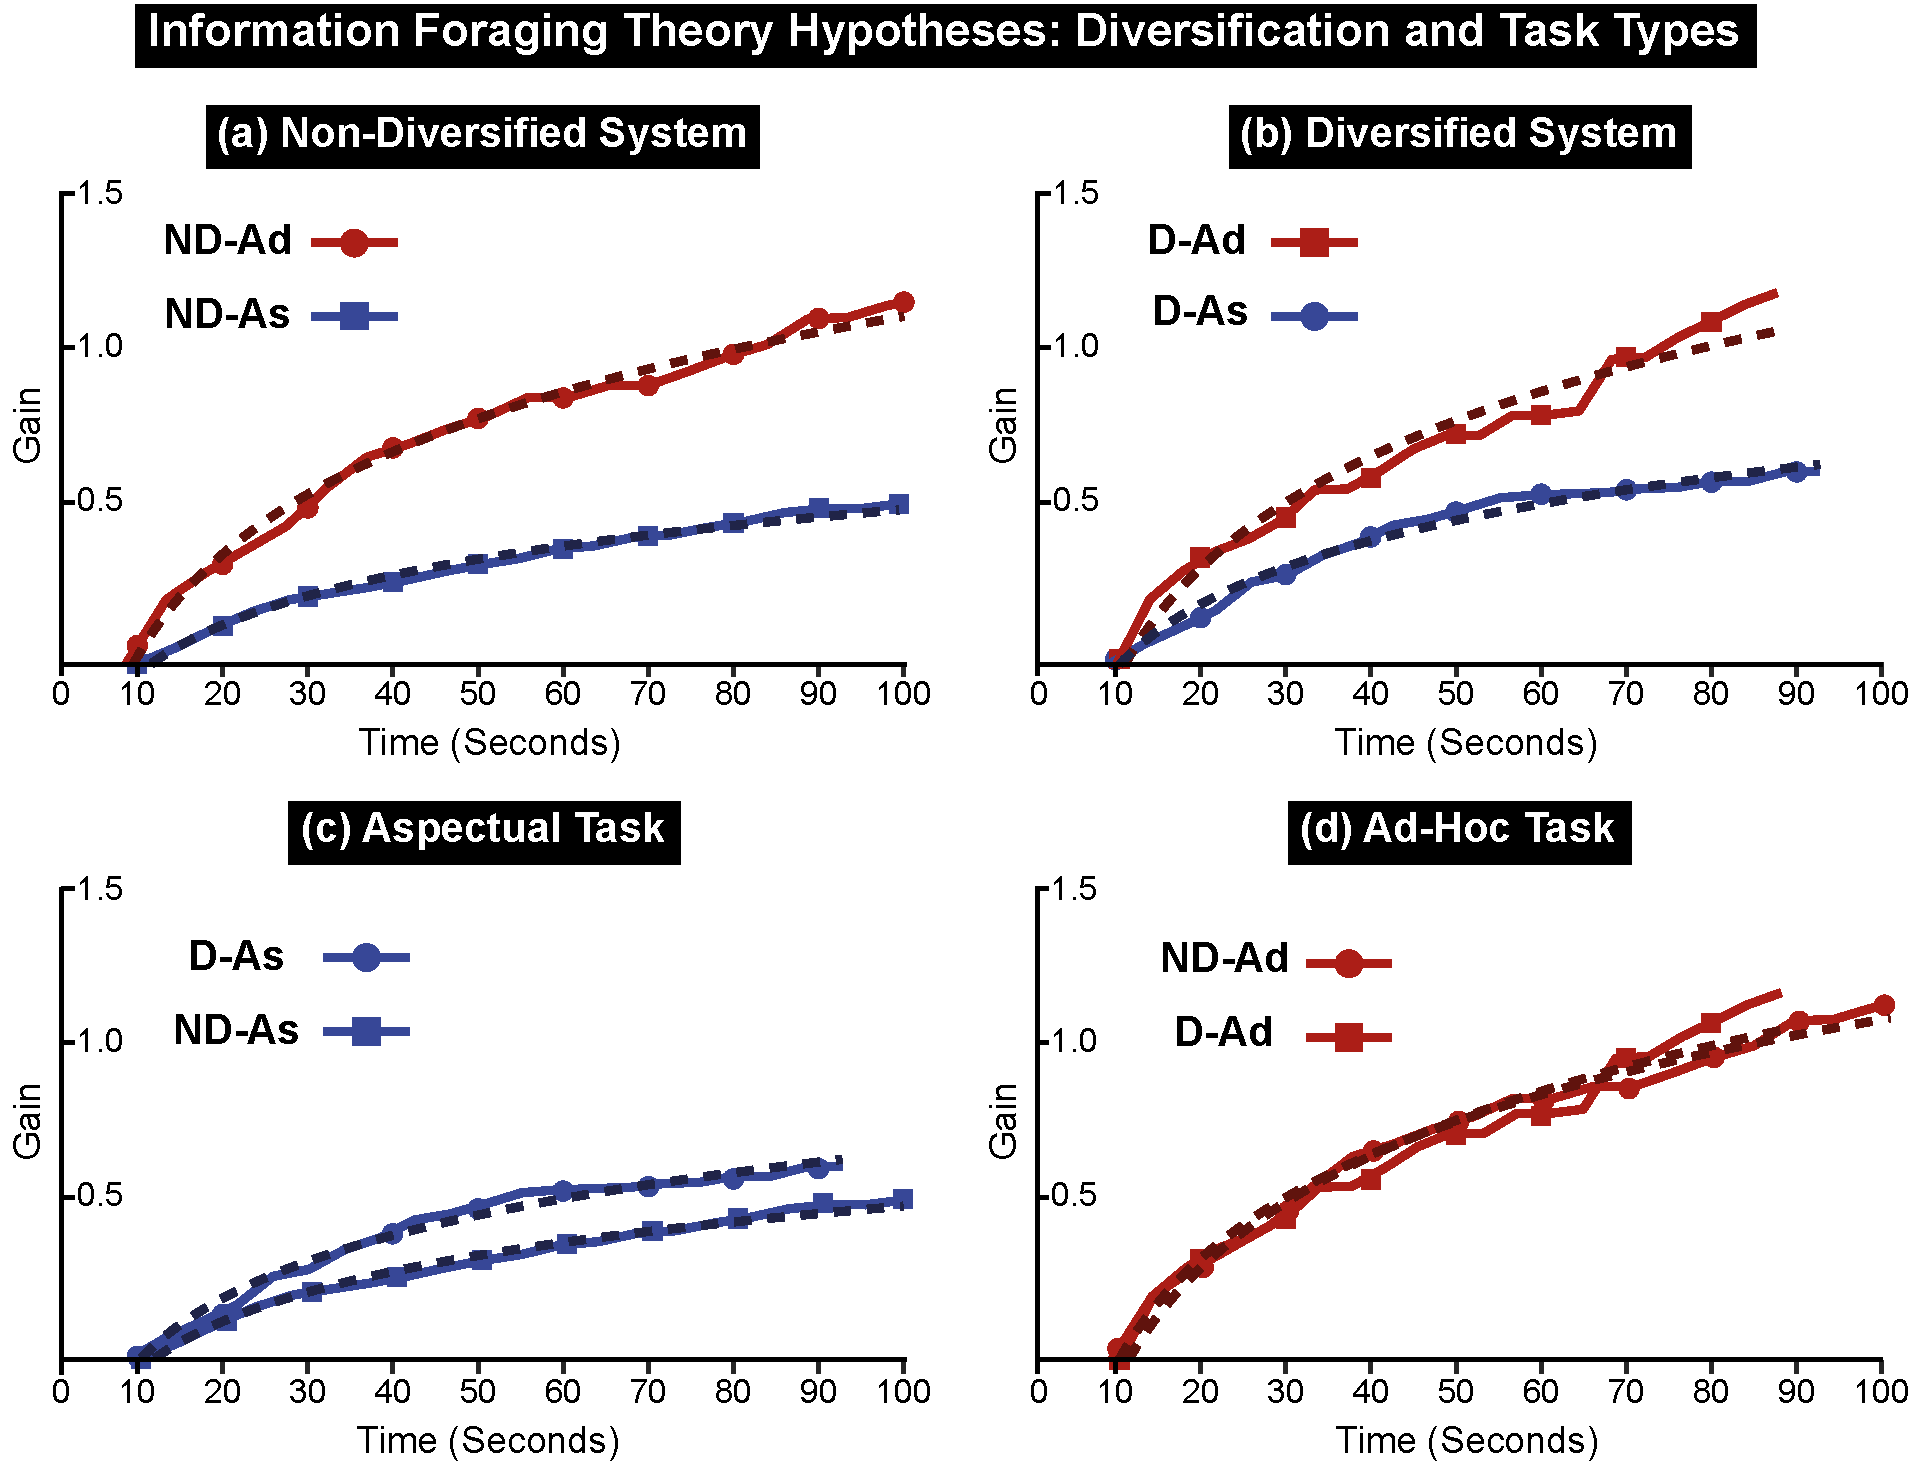
\includegraphics[width=\textwidth]{figures/cg-fromthesis.pdf}
\caption{Plots illustrating the \emph{Cumulative Gain (CG)} attained by subjects of the study, on average, over the first 100 seconds of a search session. Plots are analogous to those in Figure~\ref{fig_ift_patches}. Also included in are fitted curves (dashed lines).} \label{fig_cg}
\end{figure}

%%%%%%%%%%%%%%%
\subsection{Gain over Time}
%%%%%%%%%%%%%%%
We motivated this study using IFT, where we constructed a number of gain curves that reflected our beliefs about the search performance experienced by users would look like on each system and task. This was done to generate the hypotheses mentioned above. Here, we examine how participants performed over time for each of the systems and conditions to infer the gain curves. We then compare that to our expectations (which are shown in Figure~\ref{fig_ift_patches}).

To create empirical gain curves, we plotted cumulative gain over time, where we defined gain to be the number of saved relevant documents (in the case of ad-hoc retrieval), and gain to be the number of saved relevant but different documents (in the case of aspectual retrieval). These definitions are what we said would constitute a useful document in these tasks. And as they are in the same units, we can plot the gain for both tasks on the same axes.

Figure~\ref{fig_cg} shows the corresponding empirical gain curves for: \textit{(a)} the non-diversified system on both tasks, \textit{(b)} the diversified System on both tasks, \textit{(c)} the aspectual task for both systems, and \textit{(d)} the ad-hoc task for both systems. Compared to our expectations in Figure~\ref{fig_ift_patches}, on visual inspection, we see that our predictions were roughly in line with the gain experienced. For example, in \textit{(a)} we hypothesised that on the non-diversified system, participants would experience greater levels of gain, and the empirical gain curves show this. A critical difference though is for \textit{(b)} -- where we hypothesised that the gain curves would be similar on the diversified system, up until a point, before the aspectual gain would drop. From \textit{(b)}, it is clear that participants had a very different experience -- and experienced lower gains from the beginning -- motivating a revision of our expectations.

To do so, we first fit a logarithmic function to each of the gain curves given time (as done in \cite{ath2014ift}), such that:
\begin{equation}
gain = b \cdot log(time) - a.
\end{equation}

Table~\ref{tbl_plot_fitting} shows the parameters and correlation coefficients for fit ($r^2$) for each condition. We then could calculate how many documents a participant would examine by drawing the tangent line to the estimated gain functions from the origin. This resulted in the predicted number of documents examined -- which we see are in line with the actual documents examined. With respect to \textit{(b)}, we see that for the diversified system, the theory, given their performance, suggests that participants should examine more documents per query on the aspectual task than when undertaking the ad-hoc task (i.e. 4.98 to 3.36, respectively). We observed that they examined 3.48 and 3.02 documents per query -- which follows the same trend, but not the same magnitude. Thus, the revising our expectations regarding how people would search differently between these tasks. With respect to \textit{H1}, we see that the theory, given their performance, suggests that participants, when undertaking the aspectual task, would examine fewer documents per query when using the diversified system than on the non-diversified system (4.36 vs 4.92). Again, we see that they examined 3.02 and 3.65 documents per query respectively, again following the same trend -- but not the same magnitude. This post-hoc analysis has justified some of our initial hypotheses regarding how search behaviour would change under the different conditions -- but it has also led to us revising our expectations based on the observed, empirical data.

%We now turn our attention to examining the levels of gain that subjects experienced as they undertook search tasks in different experimental conditions. The aim here is to ascertain whether the graphical illustrations shown earlier in Figure~\ref{fig_ift_patches} are supported by empirical data from this study.

%As previously stated in Section~\ref{sec:questions}, the complexity of this study means that the notion of \emph{gain} -- that is, what each subject found during their search tasks -- changes depending upon the experimental condition that they partook in. Ad-hoc retrieval tasks rely only upon the notion of relevance, meaning that in the context of this study, correctly identifying and saving a TREC relevant document would lead to an increase in gain. Conversely, under the aspectual retrieval tasks, the notion here was to find relevant documents, containing at least one new aspect/entity related to the topic. As such, gain for these tasks was measured according to the number of new entities (in the context of a search session), encountered through each saved document. Using these measurements, we were then able to parse the interaction log to determine the levels of \emph{Cumulative Gain (CG)} that subjects attained, on average, over each of the different conditions trialled. The two plots in Figure~\ref{fig_cg} illustrate the levels of CG attained -- the plot on the left concerns ad-hoc retrieval tasks (conditions \textbf{\emph{D.Ad}} and \textbf{\emph{ND.Ad}}), while the plot on the right considers aspectual retrieval (conditions \textbf{\emph{D.As}} and \textbf{\emph{ND.As}}).

%From the data attained, we could also then use IFT to begin to make a series of predictions regarding the number of documents that subjects would examine and their corresponding stopping depths. Table~\ref{tbl_plot_fitting} shows the fitting parameters, with the plots in Figure~\ref{fig_cg} also including dash lines, representing the fitted curve to each data series.


\begin{table}[t]
    \caption{Fitting parameters for the gain curves illustrated in Figure~\ref{fig_cg} over each experimental condition. Also included are the estimations from the model for the time to examine a document, and the depth to which subjects should go \emph{(Pred. Docs.)} -- as well as the observed number of documents examined \emph{(Actual Docs.)}, and stopping depth (on average).}
    \label{tbl_plot_fitting}
    \renewcommand{\arraystretch}{1.4}
    \begin{center}
    \begin{small}
    \begin{tabulary}{\textwidth}{L{4.2cm}||D{1cm}|D{1cm}|D{1cm}|D{1cm}|D{1cm}}
    %\begin{tabulary}{\textwidth}{c||c|c|c|c|c}
    
    \hline
    
    % OUTPUT FROM script

& \multicolumn{3}{c|}{\textbf{Model Fitting}} & \textbf{Pred.} & \textbf{Actual} \\

\textbf{Experimental Condition} & \boldmath{$a$} & \boldmath{$b$} & \boldmath{$r^2$} &  \hspace*{-0.5mm}\textbf{Docs.} & \hspace*{-0.5mm}\textbf{Docs.}\\ \hline\hline

\textbf{\emph{ND.Ad}} & $-1.08$ & $0.48$ & $0.989$ & $3.68$ & $3.23$  \\ \hline
\textbf{\emph{ND.As}} & $-0.57$ & $0.23$ & $0.987$ & $4.92$ & $3.65$  \\ \hline\hline
\textbf{\emph{D.Ad}} & $-1.22$ & $0.52$ & $0.959$ & $4.98$ & $3.48$  \\ \hline
\textbf{\emph{D.As}} & $-0.68$ & $0.29$ & $0.985$ & $4.36$ & $3.02$  \\ \hline
    % END OUTPUT
    \end{tabulary}
    \end{small}
    \end{center}
\end{table}


%!TEX root = jir2018aspects.tex
\section{Summary and Conclusions} \label{sec:conclusion}

In this paper, we investigated the effects of diversifying search results when searchers undertook complex search tasks, requiring one to learn about different aspects of a topic. We inferred a number of hypotheses based upon IFT, in which diversification would lead to searchers examining fewer documents per query, and subsequently issuing more queries. We tested our hypotheses by conducting a within-subjects user study, using \emph{(i)} a non-diversified system; versus \emph{(ii)} a diversified system, when the retrieval task was either: \emph{(a)} ad-hoc; or \emph{(b)} aspectual in nature.

Our findings lend evidence to support the IFT hypotheses broadly; though we only observed statistically significant differences across a subset of behaviourial and temporal measures. This was despite the fact that there were significant differences in the performance of the two systems i.e. the diversified system was able to on average return a ranked list of results with a greater number of documents containing new, unseen entities. This finding though is in line with past work, which found that interface based interventions seemingly had little influence on search performance and search behaviours. Clearly, bigger differences  need to be present  or a larger sample size is required to determine if the difference between systems over all indicators is significant. However, there were a number of clear trends.

When performing the aspectual task on the Diversified system (in contrast to the Non-Diversified System):  participants examined fewer documents per query (3 vs. 3.7 documents/query), issued slightly fewer queries (5.9 vs. 5.2 queries), and didn't go to as great a depth when examining SERPs (depths of 12.8 vs 15.7). Taken together this resulted in a lower probability of clicking ( $P(C)$ = 0.16 vs 0.21, which was significantly different) and interestingly a lower probability of clicking on non-relevant ($P(C|N)$ = 0.13 vs. 0.18, which was also significantly different). While participants spent a similar amount of time searching on both systems, participants on the diversified system spent slightly more time examining each document (16 seconds vs. 13 seconds), and more time in total examining documents (163 seconds vs. 145 seconds) - suggesting that more effort was directed to assessing rather than searching. However, participants found significantly more entities (7.2 vs. 4.3 entities), and found more documents that contained new / different entities (3.2 vs 2.4). Both of these findings were statistically significant. This shows that the diversification algorithm led to a greater awareness of the topics and provided participants with greater coverage of the topic - which suggests that participants were able to learn more about the topic, and were exposed to less bias.

When performing the ad-hoc task on the Diversified system (in contrast to the Non-Diversified System): participants examined more documents per query (3.48 vs. 3.23 documents/query), issued slightly more queries (4.96 vs. 5.20 queries), and examined content to greater depths presented on SERPs (depths of 16.2 vs. 13.9). Again, this meant that the probability of clicking was lower on the diversified system (0.16 vs. 0.20); and this was significantly so. Participants again here spent similar amounts of time searching on both systems. However, unlike on the aspectual tasks, participants spent less time examining potentially relevant documents on the non-diversified system (13.7 vs. 15.1 seconds) and they spent less time in total assessing documents (139.6 vs, 152.8 seconds) - suggesting that less effort was directed to assessing than searching. Possibly this is because the performance of the diversified system was higher than on the non-diversified system (P@5=0.29 vs. 0.25, which was significantly different). Or perhaps the results returned were easier to identify as relevant as the probability of marking a document given it was relevant was higher (0.74 vs. 0.67). This suggests that participants may be more confident when using the diversified system. In terms of finding entities, although not explicitly requested in the task description, participants encountered more novel entities when using the diversified system (5.8 vs. 4.4). Participants also found more documents with new entities using the diversified system (2.6 vs. 2.0). Taken together this suggests that participants again learn more about the topic, implicitly, because the diversified system surfaced content that presented a more varied view on the topic.

%More relevant documents were found, and more new entities were found, suggesting they found out more about the topics on the diversified system. They also inspected fewer non-relevant documents. 

With regards to the application of IFT, we showed that generated hypotheses were largely sound, but the empirical data prompted us to revise the hypotheses . Initially, we hypothesized that the performance and behaviour on both tasks would be similar  when using the diversified system (see Fig.~\ref{fig_ift_patches}(b)). However, the post-hoc analysis revealed that the performance (and subsequent behaviour) was different (see Fig.~\ref{fig_cg}(b)), where participants obtained higher levels gain for the ad-hoc task. And thus, under such conditions, IFT would stipulate that they would examine more documents per query (3.48 vs 3.02 documents/query), and thus issued fewer queries (4.9 vs. 5.9 queries) when undertaking the ad-hoc retrieval task vs. the aspectual retrieval task (as opposed to there being no difference). Encouragingly, our application of IFT, before and after the experiment, led to new insights into how behaviours are affected under the different conditions -- show that IFT is a useful tool in developing, motivating and analysing search performance and behaviours. Furthermore, counter to our intuition about how we \emph{believed} people would behave in these conditions, the theory provided more informed and accurate hypotheses - which tended to hold in practice.



\todo{Future work}
This work motivates further research into complex search tasks and the impact of diversifying search results. That is because diversification can play an important role in improving the search experience, by providing greater coverage of a topic and mitigating potential bias in search results. One such avenue is a per-topic analysis. As our results were presented as a mean over each experimental condition (or system, or task, as reported in the bottom table of Table~\ref{tbl_actions}, we may have been largely ignorant of per-topic differences. For example, a large variance in the number of different entities identified for each topic were observed (e.g. Airport Security has 14 different airports identified, with 168 different species of animal identified for the Wildlife Extinction topic). However, a low variance in the number of entities found (see Table~\ref{tbl_actions}) suggests that this may not actually be the case. Further work includes an investigation into how such behaviours vary with a larger number of participants (increased experimental power), and how such behaviours vary under different retrieval tasks and search contexts. Would different retrieval tasks affect the perceptions of individuals and their decisions? Finally, an examination of different retrieval algorithms would provide us with a better understanding of how these influence searchers.

% ----- stay up there ------

In conclusions, we found that in terms of search behaviour: participants on the diversified system issued more queries and examined fewer documents per query, when perform the aspectual search task. Furthermore, we showed that when using the diversified system, participants were: more successful in marking relevant documents, and obtained a greater awareness of the topics (i.e. identified relevant documents containing novel aspects). This was also the case, even when they were not specifically instructed to do so, i.e. when performing the ad-hoc search task.
These findings suggest that diversification should be employed more widely -- in particular in the context of news search -- where bias is an issue, and diversification algorithms can present a broader overview of the aspects within a topic.   



%This study motivates further research in the influe

%Despite this, however, the subjects of this study found it difficult to discern the difference between the two systems, suggesting that searchers don't really notice whether a set of results have been diversified or not. Indeed, regardless of whether or not results were diversified, performance of the subjects remained similar across the two systems. Subjects did identify more entities using the diversified system -- but still performed well without it. Searchers are able to adapt their behaviour to extract a decent level of performance out, regardless of the search task and system that they are using.



\vspace*{4mm}
\noindent\textbf{Acknowledgements} The authors would like to thank the 51 Amazon Mechanical Turk Workers for their participation in the study. We would also like to thank the anonymous reviewers for their insightful feedback related to the initial submission of this article. The lead author would also like to acknowledge support from the EPSRC, grant number \texttt{1367507}.

%\bibliographystyle{spbasic}
\bibliographystyle{spmpsci} 
\bibliography{references}



%\begin{acknowledgements}
%If you'd like to thank anyone, place your comments here
%and remove the percent signs.
%\end{acknowledgements}

% BibTeX users please use one of
%\bibliographystyle{spbasic}      % basic style, author-year citations
%\bibliographystyle{spmpsci}      % mathematics and physical sciences
%\bibliographystyle{spphys}       % APS-like style for physics
%\bibliography{}   % name your BibTeX data base

% Non-BibTeX users please use
%\begin{thebibliography}{}
%
% and use \bibitem to create references. Consult the Instructions
% for authors for reference list style.
%
%\bibitem{RefJ}
% Format for Journal Reference
%Author, Article title, Journal, Volume, page numbers (year)
% Format for books
%\bibitem{RefB}
%Author, Book title, page numbers. Publisher, place (year)
% etc
%\end{thebibliography}

\end{document}
% end of file template.tex

